\documentclass[12pt,a4paper,oneside]{report}

% --- GÓI NGÔN NGỮ VÀ FONT CHỮ ---
\usepackage{fontspec}
\setmainfont{Times New Roman}
\usepackage[vietnamese]{babel}
\sloppy
\hyphenpenalty=10000
\exhyphenpenalty=10000

% --- ĐỊNH DẠNG TRANG VÀ GIÃN DÒNG ---
\usepackage{geometry}
\geometry{
  a4paper,
  left=3.0cm,
  right=2.0cm,
  top=2.5cm,
  bottom=2.5cm
}
\usepackage{setspace}
\setstretch{1.3}
\usepackage{indentfirst}
\setlength{\parindent}{0.8cm}
\setlength{\parskip}{3pt}

% --- TOÁN HỌC VÀ KÝ HIỆU ---
\usepackage{amsmath, amssymb, amsthm}

% --- MÀU SẮC VÀ ĐỒ HỌA ---
\usepackage{xcolor}
\definecolor{navy}{RGB}{0, 40, 100}
\definecolor{darkblue}{RGB}{0, 0, 139}
\definecolor{teal}{RGB}{0, 110, 110}
\definecolor{darkred}{RGB}{150, 0, 0}
\definecolor{graytext}{RGB}{80, 80, 80}

\usepackage{graphicx}
\usepackage{tikz}
\usetikzlibrary{arrows.meta, positioning, calc, shapes.geometric, backgrounds}
\usepackage{tcolorbox}
\tcbuselibrary{skins, breakable}

% --- BẢNG BIỂU ---
\usepackage{booktabs}
\usepackage{tabularx}
\usepackage{array}
\usepackage{multirow}

% --- TIÊU ĐỀ MỤC VÀ ĐỊNH DẠNG CHƯƠNG ---
\usepackage{titlesec}
\titleformat{\chapter}[display]
  {\normalfont\Large\bfseries\color{navy}}
  {\filleft\large\MakeUppercase{\chaptertitlename} \Huge\thechapter}
  {1ex}
  {\titlerule[1.5pt]\vspace{1ex}\filcenter\huge\MakeUppercase}
  [\vspace{1ex}{\color{navy}\titlerule[0.8pt]}]

\titleformat{\section}
  {\normalfont\large\bfseries\color{navy}}
  {\thesection}{1em}{}

\titleformat{\subsection}
  {\normalfont\normalsize\bfseries\color{darkblue}}
  {\thesubsection}{1em}{}

\titlespacing*{\chapter}{0pt}{0pt}{20pt}
\titlespacing*{\section}{0pt}{14pt}{8pt}
\titlespacing*{\subsection}{0pt}{10pt}{6pt}

% --- ĐẦU TRANG VÀ CHÂN TRANG ---
\usepackage{fancyhdr}
\setlength{\headheight}{15pt}
\addtolength{\topmargin}{-3pt}
\pagestyle{fancy}
\fancyhf{}
\fancyhead[L]{\small\itshape\color{graytext} Báo cáo môn học: Các mô hình toán ứng dụng}
\fancyhead[R]{\small\itshape\color{graytext} ĐHQGHN -- Trường ĐH Khoa học Tự nhiên}
\fancyfoot[C]{\thepage}
\renewcommand{\headrulewidth}{0.5pt}
\renewcommand{\footrulewidth}{0pt}

% --- LIÊN KẾT VÀ THAM CHIẾU ---
\usepackage{cite}
\usepackage[unicode]{hyperref}
\hypersetup{
  pdftitle={Báo cáo môn học: Ứng dụng mô hình Lotka–Volterra mở rộng cho hệ sinh thái Atlantic Menhaden – Striped Bass},
  pdfauthor={Tạ Tiến Nam, Tạ Văn Nghĩa, Trần Đức Kiên (K68A2)},
  pdfsubject={Các mô hình toán ứng dụng},
  colorlinks=true,
  linkcolor=navy,
  citecolor=teal,
  urlcolor=navy,
  bookmarksnumbered=true
}

% --- MÔI TRƯỜNG TOÁN HỌC ---
\newtheorem{dinhly}{Định lý}[chapter]
\newtheorem{dinhnghia}{Định nghĩa}[chapter]
\newtheorem{bode}{Bổ đề}[chapter]
\newtheorem{menhde}{Mệnh đề}[chapter]
\newtheorem{nhanxet}{Nhận xét}[chapter]

% ==============================================================================
% THÂN BÁO CÁO
% ==============================================================================
\begin{document}

% --- TRANG BÌA ---
\begin{titlepage}
\begin{tikzpicture}[remember picture, overlay]
  % Khung viền đôi trang trọng chuẩn báo cáo học thuật
  \draw[line width=3pt, color=navy] 
    ($(current page.north west) + (2.0cm,-2.0cm)$) 
    rectangle 
    ($(current page.south east) + (-1.5cm,2.0cm)$);
  \draw[line width=1pt, color=navy] 
    ($(current page.north west) + (2.15cm,-2.15cm)$) 
    rectangle 
    ($(current page.south east) + (-1.35cm,2.15cm)$);
\end{tikzpicture}

\begin{center}
  \vspace*{-0.5cm}
  {\large \textbf{ĐẠI HỌC QUỐC GIA HÀ NỘI}}\\[0.2cm]
  {\large \textbf{TRƯỜNG ĐẠI HỌC KHOA HỌC TỰ NHIÊN}}\\[0.2cm]
  {\normalsize \textbf{KHOA TOÁN -- CƠ -- TIN HỌC}}\\[0.3cm]
  \rule{5cm}{0.8pt}\\[0.6cm]

  % VỊ TRÍ ĐẶT LOGO TRƯỜNG ĐHKHTN (logo_hus.png)
  \IfFileExists{logo_hus.png}{%
    
\includegraphics[height=5.2cm, keepaspectratio]{logo_hus.png}\\[0.6cm]
  }{%
    \IfFileExists{figures/logo_hus.png}{%
      \includegraphics[height=5.2cm, keepaspectratio]{figures/logo_hus.png}\\[0.6cm]
    }{%
      \begin{tikzpicture}
        \draw[dashed, thick, navy!70, rounded corners=2mm] (0,0) rectangle (4.5, 4.5);
        \node[font=\footnotesize\itshape, text=navy, align=center] at (2.25, 2.25) {Vị trí đặt Logo HUS\\[4pt]\textbf{logo\_hus.png}};
      \end{tikzpicture}\\[0.6cm]
    }%
  }

  {\large \textbf{BÁO CÁO TIỂU LUẬN MÔN HỌC}}\\[0.3cm]
  {\Large \textbf{CÁC MÔ HÌNH TOÁN ỨNG DỤNG}}\\[0.6cm]

  \begin{tcolorbox}[colback=blue!5!white, colframe=navy, arc=3mm, width=0.92\textwidth, boxrule=1.2pt]
    \centering \vspace{0.2cm}
    {\large \textbf{ĐỀ TÀI:}}\\[0.3cm]
    {\Large \bfseries \MakeUppercase{Ứng dụng mô hình Lotka–Volterra mở rộng cho hệ sinh thái Atlantic Menhaden – Striped Bass}}\\[0.4cm]
  \end{tcolorbox}

  \vspace{0.9cm}

  \begin{tabular}{p{4.5cm}ll}
    \textbf{Giảng viên hướng dẫn:} & \multicolumn{2}{l}{TS. Nguyễn Trọng Hiếu} \\[0.3cm]
    \textbf{Sinh viên thực hiện:}  & Tạ Tiến Nam   & \textbf{MSV:} 23000143 \\
                                   & Tạ Văn Nghĩa  & \textbf{MSV:} 23000145 \\
                                   & Trần Đức Kiên & \textbf{MSV:} 23000131 \\[0.3cm]
    \textbf{Lớp:}                  & \multicolumn{2}{l}{K68A2} \\
    \textbf{Khoa:}                 & \multicolumn{2}{l}{Toán -- Cơ -- Tin học} \\
  \end{tabular}

  \vfill
  {\large \textbf{Hà Nội -- 2026}}
\end{center}
\end{titlepage}


% --- CÁC TRANG MỞ ĐẦU (ĐÁNH SỐ LA MÃ) ---
\pagenumbering{roman}
\setcounter{page}{1}

% Tóm tắt nội dung
\begin{center}
  {\Large \bfseries TÓM TẮT NỘI DUNG}
\end{center}
\vspace{0.5cm}

Việc khai thác và sử dụng bền vững các nguồn tài nguyên sinh học biển đóng vai trò đặc biệt quan trọng trong việc bảo tồn đa dạng sinh học và phát triển kinh tế lâu dài, bởi việc khai thác quá mức trong thời gian dài có thể dẫn đến sự cạn kiệt trữ lượng sinh khối và đe dọa trực tiếp sự tồn vong của toàn bộ hệ sinh thái. Vịnh Chesapeake (Hoa Kỳ) là một trong những hệ sinh thái ven biển phức tạp và năng động nhất thế giới, nơi mà việc duy trì nghề cá bền vững là nhân tố then chốt cho cả sự thịnh vượng kinh tế lẫn an ninh sinh thái của toàn vùng duyên hải.

Báo cáo này nghiên cứu và tái hiện toàn diện bài báo khoa học \textit{``Bioeconomic analysis of harvesting within a predator--prey system: A case study in the Chesapeake Bay fisheries''} của Iordanka N. Panayotova, John Herrmann và Nathan Kolling (công bố trên tạp chí \textit{Ecological Modelling}, 2023). Nghiên cứu xây dựng mô hình toán học dựa trên hệ sinh thái để phân tích động lực học quần thể có khai thác của hai loài cá trọng yếu trong vịnh Chesapeake: cá mòi dầu Đại Tây Dương (\textit{Brevoortia tyrannus}) đóng vai trò là con mồi (\textit{prey}) và cá vược sọc (\textit{Morone saxatilis}) đóng vai trò là động vật săn mồi (\textit{predator}).

Mô hình sử dụng hệ phương trình vi phân Lotka--Volterra tổng quát phi tuyến, được hiệu chỉnh và khớp tham số với chuỗi dữ liệu thực tế về độ phong phú cá thể từ năm 1995 đến năm 2017. Báo cáo phân tích tính đặt đúng về mặt sinh học của mô hình (tính dương và tính bị chặn của nghiệm trong miền bất biến $\Omega$), thiết lập các điều kiện tồn tại và ổn định của các điểm cân bằng kinh tế sinh thái (bionomic equilibria). Đặc biệt, nghiên cứu đi sâu so sánh ba chiến lược quản lý khai thác chủ chốt:
\begin{enumerate}
    \item \textbf{Sản lượng bền vững tối đa (MSY - Maximum Sustainable Yield):} Tối đa hóa sản lượng sinh khối bắt được trong điều kiện duy trì trữ lượng quần thể.
    \item \textbf{Sản lượng kinh tế tối đa (MEY - Maximum Economic Yield):} Tối đa hóa lợi nhuận ròng (tô kinh tế) từ việc khai thác sau khi trừ chi phí.
    \item \textbf{Sản lượng tối đa hóa độ đàn hồi sinh thái (RMY - Resilience Maximizing Yield):} Chiến lược quản lý ưu tiên khả năng tự phục hồi nhanh nhất của hệ thống về trạng thái cân bằng sau những nhiễu loạn môi trường.
\end{enumerate}

Cuối cùng, phương pháp vi phân trực tiếp được áp dụng để phân tích độ nhạy cục bộ của các tham số động thái, qua đó xác định các yếu tố có tác động chi phối mạnh nhất đến trữ lượng hai loài cá. Các kết quả này cung cấp luận cứ toán học định lượng vững chắc giúp các nhà hoạch định chính sách cân bằng hài hòa giữa lợi ích kinh tế trước mắt và mục tiêu bảo tồn hệ sinh thái bền vững trong dài hạn.

\vspace{0.4cm}
\noindent \textbf{Từ khóa:} Mô hình hóa toán học, Phương trình vi phân phi tuyến, Hệ động lực con mồi -- kẻ săn mồi, Vịnh Chesapeake, Kinh tế sinh thái (Bioeconomics), Sản lượng bền vững tối đa (MSY), Sản lượng kinh tế tối đa (MEY), Sản lượng tối đa hóa độ đàn hồi (RMY), Phân tích độ nhạy.

\vspace{1cm}
\hrule
\vspace{0.8cm}

\begin{center}
  {\Large \bfseries ABSTRACT}
\end{center}
\vspace{0.5cm}

Sustainable use of biological resources is very important as over-exploitation in the long run may lead to stock depletion, which in turn may threaten biodiversity. The Chesapeake Bay is an extremely complex ecosystem, and sustainable harvesting of its fisheries is essential both for the ecosystem's biodiversity and economic prosperity of the area. In this report, based on the research by Iordanka N. Panayotova, John Herrmann, and Nathan Kolling (published in \textit{Ecological Modelling}, 2023), we investigate an ecosystem-based mathematical modeling framework to study the population dynamics with harvesting of two key fish species in the Chesapeake Bay: the Atlantic Menhaden (\textit{Brevoortia tyrannus}) as prey and the Striped Bass (\textit{Morone saxatilis}) as predator.

The study fits the generalized Lotka--Volterra model to actual time series abundance data of the two species obtained from fisheries in the Bay from 1995 to 2017. Conditions for the existence of bioeconomic equilibria are derived, and the stability and resilience of the biological system are comprehensively investigated. Three fundamental harvesting policies are analyzed and compared: Maximum Sustainable Yield (MSY), Maximum Economic Yield (MEY), and Resilience Maximizing Yield (RMY), highlighting their long-term effects on fisheries sustainability. Furthermore, local sensitivity analysis using the direct differential method identifies the key biological parameters governing the population dynamics. This mathematical framework provides actionable insights for policymakers seeking to balance economic returns with ecosystem conservation in multi-species marine fisheries.

\vspace{0.4cm}
\noindent \textbf{Keywords:} Mathematical modeling, Differential equations, Predator--prey dynamics, Chesapeake Bay fisheries, Bioeconomics, Maximum sustainable yield, Maximum economic yield, Resilience maximizing yield, Sensitivity analysis.

\newpage

% Mục lục
\tableofcontents
\newpage

% Danh mục hình vẽ
\listoffigures
\addcontentsline{toc}{chapter}{Danh mục hình vẽ}
\newpage

% Danh mục ký hiệu và từ viết tắt
\chapter*{DANH MỤC KÝ HIỆU VÀ TỪ VIẾT TẮT}
\addcontentsline{toc}{chapter}{Danh mục ký hiệu và từ viết tắt}

\section*{1. Ký hiệu toán học và biến trạng thái}

\begin{table}[h!]
\centering
\begin{tabularx}{\textwidth}{l l X}
\toprule
\textbf{Ký hiệu} & \textbf{Đơn vị / Miền giá trị} & \textbf{Ý nghĩa sinh học / toán học} \\
\midrule
$t$ & Năm (Years) & Biến thời gian trong mô hình động thái quần thể \\
$x(t)$ & $10^9$ cá thể & Sinh khối / Mật độ quần thể cá mòi dầu (\textit{Atlantic menhaden} -- con mồi) \\
$y(t)$ & $10^9$ cá thể & Sinh khối / Mật độ quần thể cá vược sọc (\textit{Striped bass} -- động vật săn mồi) \\
$r$ & $\text{năm}^{-1}$ & Tốc độ tăng trưởng nội tại của quần thể con mồi \\
$a$ & $\text{năm}^{-1} \times (\text{tỷ con})^{-1}$ & Hệ số tự giới hạn (cạnh tranh nội bộ loài) của con mồi \\
$b$ & $\text{năm}^{-1} \times (\text{tỷ con})^{-1}$ & Tỷ lệ cá mòi dầu bị cá vược sọc săn bắt (tác động của kẻ săn mồi) \\
$e$ & $\text{năm}^{-1}$ & Tỷ lệ tử vong tự nhiên của cá vược sọc khi không có con mồi \\
$c$ & $\text{năm}^{-1} \times (\text{tỷ con})^{-1}$ & Hệ số tự giới hạn (cạnh tranh nội bộ loài) của kẻ săn mồi \\
$d$ & $\text{năm}^{-1} \times (\text{tỷ con})^{-1}$ & Hiệu suất chuyển đổi dinh dưỡng thức ăn thành sinh khối cá vược sọc \\
$E_1, E_2$ & Không thứ nguyên & Nỗ lực khai thác đánh bắt đối với cá mòi dầu và cá vược sọc \\
$q_1, q_2$ & $[0, 1]$ & Hệ số khả năng đánh bắt (\textit{catchability coefficients}) của từng loài \\
$p_1, p_2$ & Đơn vị tiền tệ / sinh khối & Giá bán trên một đơn vị sinh khối của từng loài \\
$c_1, c_2$ & Đơn vị tiền tệ / nỗ lực & Chi phí vận hành trên một đơn vị nỗ lực khai thác của từng loài \\
$\pi(E_1, E_2)$ & Đơn vị tiền tệ / năm & Hàm tô kinh tế (lợi nhuận ròng hàng năm từ khai thác) \\
$\tau$ & Năm & Thời gian hồi phục của hệ sinh thái về trạng thái cân bằng \\
$R$ & $\text{năm}^{-1}$ & Độ đàn hồi / độ hồi phục sinh học (\textit{Resilience}), $R = 1/\tau = -\mathrm{Re}(\lambda_m)$ \\
$\Omega$ & Miền không gian pha & Miền bất biến dương sinh học của hệ phương trình vi phân \\
$S$ & Không thứ nguyên & Sai số chuẩn phần dư trong quá trình hồi quy phi tuyến \\
\bottomrule
\end{tabularx}
\end{table}

\section*{2. Các từ viết tắt chuyên ngành}

\begin{table}[h!]
\centering
\begin{tabularx}{\textwidth}{l l X}
\toprule
\textbf{Từ viết tắt} & \textbf{Tên tiếng Anh} & \textbf{Ý nghĩa tiếng Việt} \\
\midrule
\textbf{MSY} & Maximum Sustainable Yield & Sản lượng bền vững tối đa \\
\textbf{MEY} & Maximum Economic Yield & Sản lượng kinh tế tối đa \\
\textbf{RMY} & Resilience Maximizing Yield & Sản lượng tối đa hóa độ đàn hồi sinh thái \\
\textbf{CPUE} & Catch Per Unit Effort & Sản lượng đánh bắt trên một đơn vị nỗ lực \\
\textbf{EBFM} & Ecosystem-Based Fisheries Management & Quản lý nghề cá dựa trên hệ sinh thái \\
\textbf{ERP} & Ecological Reference Point & Điểm tham chiếu sinh thái \\
\textbf{ASMFC} & Atlantic States Marine Fisheries Commission & Ủy ban Nghề cá Biển các Bang Đại Tây Dương \\
\textbf{SEDAR} & Southeast Data, Assessment, and Review & Cơ quan Đánh giá Dữ liệu Trữ lượng Đông Nam Hoa Kỳ \\
\textbf{NEFSC} & Northeast Fisheries Science Center & Trung tâm Khoa học Nghề cá Vùng Đông Bắc Hoa Kỳ \\
\textbf{NOAA} & National Oceanic and Atmospheric Admin. & Cơ quan Quản lý Khí quyển và Đại dương Quốc gia Mỹ \\
\textbf{CBF} & Chesapeake Bay Foundation & Quỹ Bảo tồn Vịnh Chesapeake \\
\textbf{GDP} & Gross Domestic Product & Tổng sản phẩm quốc nội \\
\bottomrule
\end{tabularx}
\end{table}

\newpage

% --- CÁC CHƯƠNG CHÍNH (ĐÁNH SỐ A-RẬP) ---
\pagenumbering{arabic}
\setcounter{page}{1}

% Chương 1: Mở đầu
\chapter{MỞ ĐẦU}
\label{ch:introduction}

\section{Bối cảnh nghiên cứu và hệ sinh thái vịnh Chesapeake}
\label{sec:intro_chesapeake}

Việc khai thác và quản lý bền vững các nguồn tài nguyên thiên nhiên tái tạo, đặc biệt là nguồn lợi thủy sản biển, hiện đang là một trong những thách thức liên ngành cấp bách nhất đối với toán học ứng dụng, sinh thái học và kinh tế học môi trường. Khi các hoạt động khai thác vượt quá ngưỡng chịu đựng tự nhiên của quần thể sinh vật, tình trạng cạn kiệt nguồn lợi sinh khối (\textit{stock depletion}) sẽ xảy ra trong dài hạn, kéo theo sự đổ vỡ của chuỗi thức ăn tự nhiên và đe dọa nghiêm trọng đến đa dạng sinh học toàn cầu.

Vịnh Chesapeake (nằm ở bờ biển phía Đông nước Mỹ, tiếp giáp các bang Virginia và Maryland) là vùng cửa sông (\textit{estuary}) lớn nhất tại Bắc Mỹ và là một trong những hệ sinh thái biển ven bờ phong phú nhưng có độ nhạy cảm sinh thái cao bậc nhất trên thế giới. Vịnh đóng vai trò là môi trường sống thiết yếu cho hơn 3.600 loài thực vật và động vật, đồng thời là ngư trường truyền thống cung cấp sinh kế cho hàng triệu người dân duyên hải. Để duy trì sự thịnh vượng kinh tế song hành cùng việc bảo tồn tính toàn vẹn của hệ sinh thái, việc xây dựng các chính sách khai thác nghề cá có cơ sở khoa học định lượng vững chắc là nhiệm vụ mang tính sống còn đối với các nhà quản lý \cite{panayotova2023bioeconomic}.

Trong các mô hình sinh thái học truyền thống, các quần thể sinh vật thường được xem xét dưới góc độ đơn loài (\textit{single-species management}), bỏ qua các mối tương tác cạnh tranh và săn bắt đa chiều trong lưới thức ăn. Tuy nhiên, trong môi trường tự nhiên như vịnh Chesapeake, sự biến động số lượng của một loài mắt xích có thể gây ra những hiệu ứng dây chuyền (\textit{trophic cascade}) làm đảo lộn cấu trúc của toàn bộ hệ sinh thái. Bài báo khoa học của Iordanka N. Panayotova, John Herrmann và Nathan Kolling (2023) \cite{panayotova2023bioeconomic} tập trung nghiên cứu mối quan hệ tương tác mật thiết giữa hai loài cá có tầm quan trọng kinh tế và sinh thái bậc nhất tại vịnh Chesapeake:
\begin{enumerate}
    \item \textbf{Cá mòi dầu Đại Tây Dương} (\textit{Brevoortia tyrannus} -- Atlantic Menhaden): loài cá mồi (\textit{prey}) chiếm sinh khối khổng lồ, đóng vai trò nền tảng dinh dưỡng của vịnh.
    \item \textbf{Cá vược sọc} (\textit{Morone saxatilis} -- Striped Bass / Rockfish): loài cá ăn thịt hàng đầu (\textit{predator}), là mục tiêu chính của các ngành kinh tế khai thác thương mại và câu cá giải trí.
\end{enumerate}

\section{Đặc điểm sinh học và vai trò của các loài sinh vật nghiên cứu}
\label{sec:intro_species}

\subsection{Cá mòi dầu Đại Tây Dương (\textit{Brevoortia tyrannus}) -- Loài cá mồi nền tảng}

Cá mòi dầu Đại Tây Dương (\textit{Brevoortia tyrannus}) được đông đảo các nhà sinh học biển và quản lý môi trường công nhận là \textit{``loài cá quan trọng nhất trong vịnh Chesapeake''} \cite{cbf2021menhaden}. 

\paragraph{Đặc điểm sinh học và tập tính:}
Cá mòi dầu trưởng thành có thể đạt chiều dài khoảng 18 inch (xấp xỉ 45 cm), tuổi thọ dao động từ 10 đến 12 năm và cân nặng trung bình lên đến 1 pound (khoảng 0.45 kg) \cite{ahrenholz1991population, cbp2021menhaden}. Chúng có tập tính bơi thành những đàn khổng lồ (\textit{schools}) với mật độ dày đặc tại các tầng nước mặt ven bờ và cửa sông. Hoạt động sinh sản diễn ra chủ yếu vào các tháng thời tiết mát mẻ hoặc lạnh trong năm, song trên thực tế chúng có khả năng sinh sản rải rác quanh năm tại các vùng nước biển ấm hơn \cite{ahrenholz1991population, ahrenholz1987population}.

\paragraph{Cơ chế dinh dưỡng và vai trò làm sạch môi trường nước:}
Cá mòi dầu là sinh vật ăn lọc (\textit{filter-feeder}). Cấu tạo mang của chúng có các lược mang (\textit{gill rakers}) rất phát triển và mịn màng, hoạt động như một hệ thống lưới lọc cơ học hoàn hảo giúp chúng lọc các hạt thức ăn lơ lửng trong nước khi bơi mở miệng. Chế độ dinh dưỡng của cá mòi dầu bao gồm thực vật phù du (\textit{phytoplankton}), động vật phù du (\textit{zooplankton}) và các vụn bã thực vật hữu cơ \cite{june1970food}. Thông qua việc tiêu thụ khối lượng khổng lồ tảo và sinh vật phù du, cá mòi dầu đóng vai trò như những ``nhà máy xử lý sinh học tự nhiên'', giúp hạn chế hiện tượng phú dưỡng hóa (\textit{eutrophication}), kiểm soát sự bùng phát của tảo độc và giữ cho làn nước vịnh Chesapeake luôn trong sạch và giàu dưỡng khí.

\paragraph{Mắt xích truyền tải năng lượng sinh khối:}
Về mặt chức năng sinh thái học, cá mòi dầu đóng vai trò cầu nối chuyển giao năng lượng và chất dinh dưỡng từ các bậc dinh dưỡng thấp (sinh vật sản xuất sơ cấp) lên các bậc dinh dưỡng cao hơn trong chuỗi thức ăn biển \cite{anstead2021path}. Chúng là nguồn thức ăn chính và giàu năng lượng cho hàng loạt loài sinh vật ăn thịt quan trọng trong vịnh:
\begin{itemize}
    \item Các loài cá săn mồi thương mại: cá vược sọc (\textit{Morone saxatilis}) \cite{walter2003diet}, cá xanh (\textit{Pomatomus saltatrix}) \cite{harding2001diet}, cá yếu (\textit{Cynoscion regalis}) \cite{merriner1975food}.
    \item Động vật săn mồi biển lớn: các loài cá mập cát (\textit{Carcharhinus plumbeus}) \cite{ellis2003diet}.
    \item Chim săn mồi ven biển: chim ưng biển (\textit{Pandion haliaetus} -- Osprey) \cite{glass2009osprey}, đại bàng đầu trắng.
    \item Các loài động vật có vú biển và chim di cư ven bờ.
\end{itemize}

\paragraph{Giá trị kinh tế và sức khỏe con người:}
Bên cạnh vai trò sinh thái, cá mòi dầu tạo ra nguồn lợi kinh tế khổng lồ. Mặc dù thịt của cá mòi dầu nhiều xương và dầu, không phù hợp để dùng trực tiếp làm thực phẩm trên bàn ăn thông thường, nhưng loài cá này lại là đối nguyên liệu hàng đầu cho ngành công nghiệp chế biến bột cá (dùng làm thức ăn chăn nuôi gia súc, gia cầm và nuôi trồng thủy sản) cũng như làm mồi câu cho nghề đánh bắt cua xanh và tôm hùm. Đặc biệt, dầu ép từ cá mòi dầu rất giàu các axit béo không bão hòa đa chuỗi dài Omega-3 (đặc biệt là EPA và DHA). Các hợp chất này có giá trị y dược và dinh dưỡng cực kỳ cao, hỗ trợ giảm thiểu nguy cơ mắc các bệnh tim mạch, viêm khớp và tăng cường chức năng não bộ ở con người.

\subsection{Cá vược sọc (\textit{Morone saxatilis}) -- Kẻ săn mồi đầu bảng}

Cá vược sọc (\textit{Morone saxatilis}), thường được gọi dân dã là \textit{Rockfish}, là một trong những loài cá biểu tượng và có giá trị cao nhất tại vùng vịnh Chesapeake cũng như toàn bộ vùng duyên hải Đại Tây Dương của Bắc Mỹ \cite{cbp2021stripedbass}.

\paragraph{Đặc điểm sinh học và vòng đời:}
Cá vược sọc trưởng thành có kích thước lớn, chiều dài phổ biến từ 2 đến 3 feet (khoảng 60 đến 90 cm) và khối lượng dao động từ 10 đến 30 pounds (tương đương 4.5 đến 13.6 kg), đôi khi có những cá thể vượt quá 40--50 pounds. Đây là loài cá di cư sinh sản ngược dòng (\textit{anadromous}): chúng sống phần lớn cuộc đời trưởng thành ở vùng nước lợ và biển, nhưng di cư ngược dòng vào vùng nước ngọt của các nhánh sông thuộc vịnh Chesapeake từ tháng 4 đến tháng 6 hàng năm để đẻ trứng. Cá con sau khi nở sẽ lưu trú và kiếm ăn ở các vùng cửa sông nông có độ mặn thấp trong vài năm đầu trước khi gia nhập đàn cá trưởng thành ngoài biển khơi \cite{robichaud1996spawning}.

\paragraph{Tập tính săn mồi và vị trí trong lưới thức ăn:}
Cá vược sọc là loài săn mồi cơ hội ở bậc dinh dưỡng cao. Chế độ ăn của chúng rất phong phú, nhưng cá mòi dầu Đại Tây Dương chiếm tỷ trọng vượt trội trong khẩu phần thức ăn về mặt sinh khối và năng lượng trao đổi chất \cite{walter2003diet}. Bên cạnh đó, chúng tiêu thụ thêm các loài giáp xác (cua, tôm) và cá cơm biển. Khi còn nhỏ hoặc ở giai đoạn bán trưởng thành, cá vược sọc cũng là đối tượng săn mồi của cá mập lớn và chim ưng biển \cite{ellis2003diet, glass2009osprey}. Do đó, trạng thái số lượng của cá vược sọc phản ánh trực tiếp sức khỏe sinh thái của toàn bộ hệ sinh thái vịnh.

\paragraph{Tầm quan trọng kinh tế và thể thao giải trí:}
Khác với cá mòi dầu vốn chủ yếu được đánh bắt công nghiệp chế biến bột cá, cá vược sọc là trung tâm của hai ngành kinh tế thủy sản song song:
\begin{itemize}
    \item \textbf{Nghề cá thương mại (\textit{commercial fisheries}):} Cung cấp thịt cá thương phẩm cao cấp cho các nhà hàng và chuỗi cung ứng thực phẩm tươi sống trên toàn quốc.
    \item \textbf{Nghề cá giải trí (\textit{recreational fisheries}):} Ngành du lịch câu cá giải trí thu hút hàng trăm nghìn cần thủ và du khách mỗi năm. Báo cáo phân tích kinh tế của tổ chức Southwick Associates (2019) \cite{southwick2019economic} chỉ ra rằng nghề câu cá vược sọc đóng góp hàng tỷ đô la vào Tổng sản phẩm quốc nội (GDP) của Hoa Kỳ, bảo đảm hàng chục ngàn việc làm trực tiếp và gián tiếp tại 11 bang dọc theo bờ biển Đại Tây Dương.
\end{itemize}

\section{Hiện trạng suy giảm và khủng hoảng khai thác nghề cá}
\label{sec:intro_crises}

Mặc dù có vai trò thiết yếu, cả hai quần thể cá mòi dầu và cá vược sọc đều đã và đang trải qua những giai đoạn suy thoái trầm trọng, làm dấy lên những cuộc tranh luận gay gắt giữa giới khoa học bảo tồn, các nhà hoạch định chính sách và các tập đoàn công nghiệp đánh bắt.

\subsection{Khủng hoảng suy giảm cá mòi dầu và xung đột hạn ngạch}

Từ những năm 1970 đến nay, sinh khối của cá mòi dầu Đại Tây Dương đã sụt giảm nghiêm trọng và liên tục duy trì ở mức thấp báo động \cite{cbf2021menhaden}. Sự suy thoái này bắt nguồn từ hai nhóm nguyên nhân chính:
\begin{enumerate}
    \item \textbf{Các áp lực môi trường sống suy thoái:} Ô nhiễm không khí và nguồn nước, hiện tượng nước biển ấm lên và biến đổi khí hậu toàn cầu, xâm lấn của các loài sinh vật ngoại lai, suy giảm diện tích đất ngập nước ven bờ do đô thị hóa và phân bón nông nghiệp chảy tràn tạo nên những ``vùng chết'' (\textit{dead zones}) thiếu dưỡng khí vào mùa hè.
    \item \textbf{Khai thác công nghiệp quá mức (\textit{overharvesting}):} Đây được xem là mối đe dọa trực tiếp và nguy hiểm nhất. Các đội tàu công nghiệp quy mô lớn (điển hình là tập đoàn Omega Protein) sử dụng công nghệ trinh sát đàn cá bằng máy bay phối hợp cùng lưới vây khổng lồ (\textit{purse seine nets}) để càn quét các đàn cá mòi dầu trong vịnh. Các tập đoàn lớn này liên tục vấp phải sự phản đối kịch liệt từ công chúng và các nhà bảo tồn vì nhiều lần vi phạm hoặc vận động hành lang làm suy yếu hạn ngạch đánh bắt (\textit{harvest caps}) do chính quyền quy định \cite{ress2020chesapeake, cbf2021menhaden}.
\end{enumerate}

Điều đáng chú ý là tồn tại một mâu thuẫn sâu sắc giữa quan điểm quản lý hành chính và thực tế sinh thái: Trong khi Quỹ Bảo tồn Vịnh Chesapeake (\textit{Chesapeake Bay Foundation}) và các nhà khoa học độc lập liên tục cảnh báo về sự cạn kiệt của cá mòi dầu, thì Báo cáo Đánh giá Trữ lượng năm 2019 của Ủy ban Nghề cá Biển các Bang Đại Tây Dương (ASMFC) thông qua chương trình SEDAR 69 lại đưa ra nhận định rằng \textit{``loài cá mòi dầu Đại Tây Dương hiện chưa bị khai thác quá mức và tình trạng đánh bắt quá mức không xảy ra''} \cite{sedar2020menhaden}. Nghịch lý này phản ánh sự sai lệch giữa các chỉ số tính toán đơn loài truyền thống so với nhu cầu thức ăn thực tế của toàn bộ lưới sinh thái.

\subsection{Nguy cơ suy thoái và tình trạng đánh bắt quá mức của cá vược sọc}

Đối với cá vược sọc, lịch sử sinh học cũng ghi nhận những đợt sụt giảm quần thể cận kề bờ vực tuyệt chủng vào cuối thập niên 1970 và đầu thập niên 1980, đến mức các cơ quan quản lý đã phải áp đặt lệnh cấm đánh bắt tạm thời (\textit{moratorium}) nghiêm ngặt để quần thể có cơ hội phục hồi.

Tuy nhiên, trong những năm gần đây, quần thể cá vược sọc lại một lần nữa rơi vào tình trạng nguy cấp do sự kết hợp của nhiều yếu tố bất lợi:
\begin{itemize}
    \item Ô nhiễm môi trường và độ pH suy giảm tại các khu vực bãi đẻ nước ngọt.
    \item Tình trạng suy kiệt nguồn thức ăn chính: sự suy giảm của đàn cá mòi dầu khiến cá vược sọc không đủ năng lượng dự trữ, dẫn đến tình trạng gầy yếu và bùng phát các bệnh truyền nhiễm nguy hiểm (như bệnh lao cá do vi khuẩn \textit{Mycobacteriosis}).
    \item Áp lực đánh bắt quá mức từ cả tàu cá thương mại và cần thủ giải trí. Đặc biệt, nghiên cứu sinh học ghi nhận khoảng 9\% lượng cá vược sọc bắt được rồi thả lại (\textit{catch-and-release}) trong nghề câu giải trí vẫn bị chết do sốc nhiệt độ và thương tích \cite{cbf2021rockfish}.
\end{itemize}
Theo Báo cáo Đánh giá Trữ lượng tại Hội thảo Đánh giá Trữ lượng Vùng Đông Bắc lần thứ 66 do Trung tâm Khoa học Nghề cá Đông Bắc (NEFSC) công bố, trữ lượng cá vược sọc chính thức bị xếp vào diện \textbf{bị khai thác quá mức} (\textit{overfished}) và \textbf{đang diễn ra tình trạng khai thác quá mức} (\textit{overfishing}) \cite{nefsc2019stripedbass}.

\section{Thách thức quản lý tài nguyên chung và sự chuyển dịch mô hình}
\label{sec:intro_management}

\subsection{Bi kịch của tài nguyên sở hữu chung (\textit{Tragedy of the Commons})}
Trong kinh tế học tài nguyên, các ngư trường biển tự nhiên thường là tài sản chung vô chủ hoặc thuộc sở hữu công cộng mở (\textit{common property resources}). Do thiếu quyền sở hữu tài sản tư nhân được xác định rành mạch, từng đơn vị khai thác kinh tế (ngư dân, doanh nghiệp đánh bắt) luôn có xu hướng chạy đua tối đa hóa sản lượng đánh bắt nhằm nâng cao lợi nhuận trước mắt, mà không tính đến chi phí ngoại ứng (\textit{negative externalities}) và thiệt hại dài hạn đối với khả năng tái sinh của nguồn tài nguyên sinh thái. Hiện tượng này dẫn thẳng đến tình trạng suy thoái tài nguyên chung (\textit{overexploitation}) và cạn kiệt sinh học nếu không có sự can thiệp và điều tiết chặt chẽ từ phía nhà nước thông qua các công cụ pháp lý và chính sách kinh tế \cite{finley2011all}.

\subsection{Hạn chế của phương pháp quản lý đơn loài và nhu cầu mô hình hóa đa loài}
Trong suốt nhiều thập kỷ qua, các cơ quan quản lý nghề cá thường áp dụng các mô hình đánh giá trữ lượng đơn loài (\textit{single-species stock assessment models}). Phương pháp tiếp cận này giả định rằng tốc độ gia tăng sinh khối của một loài chỉ phụ thuộc vào số lượng cá thể nội bộ của chính loài đó và nỗ lực đánh bắt của con người. 

Tuy nhiên, trong một lưới thức ăn biển tương hỗ, sự tương tác sinh thái là không thể tách rời:
\begin{quote}
\textit{``Nếu chúng ta khai thác cá mòi dầu ở mức sản lượng tối đa cho phép theo mô hình đơn loài, lượng sinh khối cá mòi dầu còn lại trong nước có thể không đủ để duy trì chuỗi thức ăn của cá vược sọc, từ đó vô tình đẩy quần thể cá vược sọc vào nguy cơ sụp đổ sinh học.''}
\end{quote}
Gần đây, các nhà nghiên cứu biển quốc tế đã nhấn mạnh sự cấp thiết phải chuyển đổi sang phương thức \textbf{Quản lý nghề cá dựa trên hệ sinh thái} (\textit{Ecosystem-Based Fisheries Management -- EBFM}) \cite{anstead2021path, howell2021combining}. Nghiên cứu của Howell và cộng sự (2021) \cite{howell2021combining} đã chỉ ra rằng, để bảo đảm nhu cầu dinh dưỡng của các loài săn mồi đỉnh cao, chỉ tiêu khai thác an toàn (Điểm tham chiếu sinh thái -- \textit{Ecological Reference Points, ERP}) cho các loài cá mồi như cá mòi dầu cần phải được cắt giảm ít nhất \textbf{40\%} so với ngưỡng tính toán bằng các mô hình đơn loài thông thường.

\section{Phương pháp tiếp cận mô hình toán học trong đề tài}
\label{sec:intro_methodology}

Để giải quyết bài toán phức tạp trên một cách khả thi và định lượng, bài báo khoa học của Panayotova và cộng sự (2023) \cite{panayotova2023bioeconomic} đã ứng dụng công cụ mô hình hóa toán học với hệ phương trình vi phân Lotka--Volterra tổng quát mở rộng.

\subsection{Hệ phương trình vi phân Lotka--Volterra hai loài}
Xét hệ hai loài tương tác gồm con mồi $x(t)$ (cá mòi dầu) và kẻ săn mồi $y(t)$ (cá vược sọc). Động thái quần thể tự nhiên được mô tả qua hệ phương trình vi phân phi tuyến:
\begin{equation}
\label{eq:intro_lv_system}
\left\{
\begin{aligned}
\frac{dx}{dt} &= x(r - ax - by), \\
\frac{dy}{dt} &= y(-e - cy + dx).
\end{aligned}
\right.
\end{equation}
Trong đó:
\begin{itemize}
    \item $r$ là tốc độ tăng trưởng nội tại của con mồi; $e$ là tốc độ tử vong tự nhiên của kẻ săn mồi khi thiếu con mồi.
    \item $a > 0$ và $c > 0$ là các hệ số tự giới hạn (\textit{self-limitation}) phản ánh sự cạnh tranh nội bộ loài (\textit{intra-species competition}) về không gian sống và thức ăn cục bộ. Giả thiết này khắc phục nhược điểm của mô hình Lotka--Volterra cổ điển (vốn dự báo dao động điều hòa không tắt) bằng cách đưa về động thái logistic tiệm cận thực tế.
    \item $b > 0$ là tỷ lệ cá mòi dầu bị cá vược sọc tiêu thụ; $d > 0$ biểu thị hiệu quả chuyển đổi dinh dưỡng từ con mồi sang tốc độ gia tăng của kẻ săn mồi.
\end{itemize}

Mặc dù mô hình \eqref{eq:intro_lv_system} là một sự tinh giản so với hệ sinh thái cực kỳ phức tạp của vịnh Chesapeake (bỏ qua cấu trúc tuổi và các tương tác với các loài sinh vật khác), nó sở hữu những ưu thế toán học vượt trội:
\begin{enumerate}
    \item \textbf{Khả năng giải tích chính xác (\textit{analytically tractable}):} Cho phép tìm tường minh các nghiệm cân bằng, phân tích tính ổn định tiệm cận của ma trận Jacobi, tính dương và tính bị chặn của nghiệm.
    \item \textbf{Mô tả được hành vi dao động lệch pha (\textit{phase-shifted behavior}):} Tái hiện chính xác hiện tượng trễ pha điển hình trong các hệ sinh thái: sự gia tăng của con mồi kích thích sự phát triển của kẻ săn mồi, sau đó áp lực săn mồi gia tăng kéo theo sự suy giảm của con mồi, và chu kỳ lặp lại.
    \item \textbf{Khả năng tích hợp dữ liệu thực nghiệm:} Số lượng tham số vừa đủ để có thể ước lượng tin cậy từ dữ liệu chuỗi thời gian thực tế mà không bị rơi vào hiện tượng quá khớp (\textit{overfitting}).
\end{enumerate}

\subsection{Sơ đồ tương tác sinh thái -- kinh tế}

Mối quan hệ qua lại giữa các yếu tố sinh thái, nguồn lợi sinh khối, hoạt động khai thác của con người và cơ chế thị trường kinh tế được tổng hợp trực quan trong Sơ đồ \ref{fig:intro_flowchart}.

\begin{figure}[h!]
\centering
\begin{tikzpicture}[
    node distance=2.5cm and 3.5cm,
    block/.style={rectangle, draw=navy, fill=blue!8, rounded corners=3mm, thick, inner sep=8pt, text width=4.5cm, align=center, font=\small\bfseries},
    harvest/.style={rectangle, draw=red!70!black, fill=red!10, rounded corners=2mm, dashed, thick, inner sep=6pt, text width=3.8cm, align=center, font=\small},
    market/.style={ellipse, draw=teal!80!black, fill=teal!10, thick, inner sep=6pt, text width=3.8cm, align=center, font=\small\bfseries},
    flow/.style={->, >=stealth, line width=1.2pt},
    eco/.style={->, >=stealth, line width=1.5pt, color=navy},
    harv/.style={->, >=stealth, line width=1.2pt, color=red!70!black, dashed}
]

% Các khối sinh thái
\node[block] (prey) {Cá mòi dầu\\(\textit{Atlantic Menhaden})\\$x(t)$ (Con mồi)};
\node[block, right=of prey] (pred) {Cá vược sọc\\(\textit{Striped Bass})\\$y(t)$ (Săn mồi)};

% Tự giới hạn
\path[eco] (prey) edge [loop above] node[above, font=\footnotesize] {Tự giới hạn $-ax^2$} (prey);
\path[eco] (pred) edge [loop above] node[above, font=\footnotesize] {Tự giới hạn $-cy^2$} (pred);

% Tương tác săn mồi
\draw[eco] (prey) -- node[above, font=\footnotesize, align=center] {Cung cấp thức ăn $(+dxy)$\\Săn bắt tiêu thụ $(-bxy)$} (pred);

% Khai thác
\node[harvest, below=1.8cm of prey] (h1) {Khai thác cá mòi dầu\\$h_1 = q_1 E_1 x$};
\node[harvest, below=1.8cm of pred] (h2) {Khai thác cá vược sọc\\$h_2 = q_2 E_2 y$};

\draw[harv] (h1) -- node[right, font=\footnotesize] {Đánh bắt} (prey);
\draw[harv] (h2) -- node[right, font=\footnotesize] {Đánh bắt} (pred);

% Kinh tế & Thị trường
\node[market, below=1.5cm of $(h1)!0.5!(h2)$] (market) {Kinh tế \& Thị trường\\Hàm tô kinh tế $\pi(E_1, E_2)$\\$R(E) - C(E)$};

\draw[flow, color=teal!80!black] (h1) |- node[below, pos=0.8, font=\footnotesize] {Doanh thu \& Chi phí} (market);
\draw[flow, color=teal!80!black] (h2) |- node[below, pos=0.8, font=\footnotesize] {Doanh thu \& Chi phí} (market);

\end{tikzpicture}
\caption{Sơ đồ tương tác sinh thái -- kinh tế trong hệ hai loài cá mòi dầu và cá vược sọc tại vịnh Chesapeake.}
\label{fig:intro_flowchart}
\end{figure}

\subsection{Tích hợp khai thác và mô hình kinh tế sinh thái (Bionomic model)}
Để nghiên cứu tác động của con người, nhóm tác giả đưa thành phần khai thác vào hệ vi phân dựa trên giả thuyết \textbf{sản lượng đánh bắt trên một đơn vị nỗ lực} (\textit{Catch-Per-Unit-Effort -- CPUE}):
\begin{equation}
h_1 = q_1 E_1 x, \quad h_2 = q_2 E_2 y.
\end{equation}
Trong đó $E_1, E_2$ là cường độ (nỗ lực) đánh bắt của các tàu thuyền đối với từng loài, và $q_1, q_2$ là các hệ số dễ đánh bắt. Kết hợp với hàm tô kinh tế (\textit{economic rent}) thể hiện lợi nhuận ròng thu được sau khi trừ chi phí đánh bắt:
\begin{equation}
\pi(E_1, E_2) = (p_1 q_1 x - c_1) E_1 + (p_2 q_2 y - c_2) E_2,
\end{equation}
với $p_i$ là đơn giá thương phẩm trên một đơn vị sinh khối và $c_i$ là chi phí cho một đơn vị nỗ lực khai thác.

\subsection{Khảo sát và đối sánh ba chính sách khai thác chiến lược}
Nghiên cứu tập trung giải quyết bài toán tối ưu hóa đa mục tiêu thông qua việc so sánh ba chính sách khai thác then chốt:
\begin{enumerate}
    \item \textbf{Chính sách Sản lượng bền vững tối đa (MSY -- Maximum Sustainable Yield):}
    Khái niệm MSY bắt nguồn từ công trình kinh điển năm 1954 của Milner B. Schaefer \cite{schaefer1954some}. Đây là cách tiếp cận nhằm xác định mức nỗ lực khai thác $E_{\mathrm{MSY}}$ để thu được sản lượng sinh khối hàng năm lớn nhất mà vẫn đảm bảo trữ lượng quần thể không bị suy giảm theo thời gian. Bài báo kiểm chứng điều kiện tồn tại của MSY trong bối cảnh hệ hai loài tương tác và chỉ ra những nguy cơ sinh học tiềm ẩn khi áp dụng máy móc MSY đơn loài cho các loài cá mồi.
    
    \item \textbf{Chính sách Sản lượng kinh tế tối đa (MEY -- Maximum Economic Yield):}
    Khác với MSY chỉ quan tâm đến sinh khối vật lý đánh bắt được, MEY nhắm tới việc tối đa hóa lợi nhuận kinh tế thuần túy $\pi(E)$. MEY xem xét yếu tố chi phí cận biên tăng dần khi nguồn cá cạn kiệt. Về mặt lý thuyết, chính sách MEY thường đòi hỏi mức nỗ lực khai thác thấp hơn MSY ($E_{\mathrm{MEY}} < E_{\mathrm{MSY}}$), do đó giúp bảo vệ quần thể cá tốt hơn và tạo ra vùng đệm an toàn trước các biến động ngẫu nhiên.
    
    \item \textbf{Chính sách Sản lượng tối đa hóa độ đàn hồi sinh thái (RMY -- Resilience Maximizing Yield):}
    Độ đàn hồi hay độ hồi phục (\textit{Resilience -- $R$}) là thước đo phản ánh tốc độ tự phục hồi của hệ thống sinh thái quay trở về trạng thái cân bằng sinh học bền vững sau khi chịu một nhiễu loạn môi trường đột ngột \cite{pimm1978feeding}. Theo lý thuyết của Pimm và Lawton (1978), thời gian phục hồi $\tau$ tỷ lệ nghịch với phần thực âm của giá trị riêng chủ đạo ($\lambda_m$) của ma trận Jacobian:
    \begin{equation}
    \tau = \frac{-1}{\mathrm{Re}(\lambda_m)}, \quad R = \frac{1}{\tau}.
    \end{equation}
    Chính sách RMY ưu tiên tối đa hóa $R$ (tức tối thiểu hóa thời gian $\tau$), đặt sự an toàn và bền vững dài hạn của cấu trúc sinh thái lên trên các mục tiêu kinh tế ngắn hạn.
\end{enumerate}

\subsection{Phân tích độ nhạy cục bộ (Sensitivity Analysis)}
Hệ thống các tham số sinh học trong thực tế thường chứa đựng những sai số đo đạc và sự biến động theo thời tiết khí hậu. Để đánh giá xem sự biến động nhỏ của từng tham số mô hình ảnh hưởng như thế nào đến nghiệm trạng thái theo thời gian, đề tài áp dụng **Phương pháp vi phân trực tiếp** (\textit{Direct Differential Method}). Bằng cách thiết lập hệ phương trình vi phân bổ sung cho ma trận độ nhạy $S_{ij} = \frac{\partial u_i}{\partial p_j}$, nghiên cứu xác định được các tham số nhạy cảm nhất, giúp các nhà quản lý tập trung nguồn lực kiểm soát đúng những mắt xích then chốt.

\section{Mục tiêu nghiên cứu và ý nghĩa của đề tài}
\label{sec:intro_objectives}

\subsection{Mục tiêu cụ thể}
Trong khuôn khổ môn học \textit{Các mô hình toán ứng dụng}, báo cáo hướng tới các mục tiêu cụ thể sau:
\begin{enumerate}
    \item \textbf{Nắm vững phương pháp mô hình hóa sinh thái học:} Hiểu rõ cơ sở toán học và sinh học của mô hình Lotka--Volterra tổng quát, ý nghĩa các tham số và các giả thiết ràng buộc.
    \item \textbf{Chứng minh chặt chẽ các tính chất toán học:} Chứng minh tính dương và tính bị chặn của nghiệm trong miền bất biến sinh học $\Omega$, tìm nghiệm cân bằng kinh tế sinh thái (bionomic equilibria) và phân tích tính ổn định cục bộ thông qua các giá trị riêng của ma trận Jacobian.
    \item \textbf{Khai thác dữ liệu thực nghiệm:} Tái hiện quy trình khớp mô hình phi tuyến với dữ liệu chuỗi thời gian giai đoạn 1995--2017 của vịnh Chesapeake, đánh giá các chỉ số sai số thống kê.
    \item \textbf{So sánh định lượng các chính sách khai thác:} Xác định tường minh công thức nghiệm cho $E_{\mathrm{MSY}}$, $E_{\mathrm{MEY}}$, $E_{\mathrm{RMY}}$ cho các kịch bản đánh bắt khác nhau (chỉ đánh bắt cá săn mồi, chỉ đánh bắt con mồi, đánh bắt hỗn hợp cả hai loài); phân tích sự đánh đổi (\textit{trade-off}) giữa lợi nhuận kinh tế và độ an toàn sinh học.
    \item \textbf{Thực hiện phân tích độ nhạy:} Đánh giá định lượng mức độ ảnh hưởng của từng tham số đến quỹ đạo nghiệm trạng thái quần thể hai loài.
\end{enumerate}

\subsection{Ý nghĩa khoa học và thực tiễn}
\begin{itemize}
    \item \textbf{Về mặt khoa học:} Báo cáo minh họa sinh động sức mạnh của toán học ứng dụng (cụ thể là lý thuyết phương trình vi phân phi tuyến, hệ động lực và giải tích ma trận) trong việc giải quyết các bài toán liên ngành phức tạp giữa kinh tế và sinh thái học.
    \item \textbf{Về mặt thực tiễn quản lý:} Kết quả nghiên cứu chứng minh rõ nét sự nguy hiểm của tư duy quản lý đơn loài đối với các loài cá mồi ven biển, đồng thời cung cấp những khuyến nghị có tính khả thi cao nhằm hỗ trợ các nhà hoạch định chính sách nghề cá vịnh Chesapeake cân đối giữa mục tiêu sinh kế và bảo tồn nguồn lợi tự nhiên.
\end{itemize}

\section{Bố cục của báo cáo}
\label{sec:intro_outline}

Báo cáo môn học được tổ chức thành 6 chương chính như sau:
\begin{itemize}
    \item \textbf{Chương 1 -- Mở đầu:} Trình bày bối cảnh nghiên cứu, tổng quan sinh học về cá mòi dầu và cá vược sọc tại vịnh Chesapeake, thực trạng khai thác, các thách thức quản lý tài nguyên chung, mô hình hóa toán học và mục tiêu của đề tài.
    \item \textbf{Chương 2 -- Mô hình toán học và dữ liệu thực tế:} Trình bày chi tiết hệ phương trình vi phân Lotka--Volterra tổng quát 2 loài, các giả thiết mô hình, phương pháp bình phương tối thiểu phi tuyến khớp với dữ liệu thời gian 1995--2017, dự báo động thái đến năm 2100 và tính toán độ đàn hồi ban đầu.
    \item \textbf{Chương 3 -- Mô hình kinh tế sinh thái và phân tích ổn định:} Xây dựng hệ bionomic có xét đến nỗ lực đánh bắt, chứng minh tính dương và tính bị chặn của nghiệm trong tập bất biến $\Omega$, xác định các điều kiện tồn tại điểm cân bằng bionomic và phân tích tính ổn định tiệm cận của hệ thống.
    \item \textbf{Chương 4 -- Phân tích các chính sách khai thác nghề cá:} Khảo sát chi tiết ba chính sách khai thác MSY, MEY và RMY trong ba kịch bản quản lý (chỉ khai thác kẻ săn mồi, chỉ khai thác con mồi, khai thác đồng thời cả hai loài); phân tích sự đánh đổi giữa lợi ích kinh tế và tính bền vững sinh thái.
    \item \textbf{Chương 5 -- Phân tích độ nhạy cục bộ:} Ứng dụng phương pháp vi phân trực tiếp để khảo sát tốc độ biến thiên của nghiệm theo 8 tham số động thái, xếp hạng các tham số then chốt chi phối hệ thống.
    \item \textbf{Chương 6 -- Thảo luận và Kết luận:} Tổng hợp các kết quả chính, thảo luận các hàm ý chính sách đối với quản lý vịnh Chesapeake, đánh giá những hạn chế của mô hình và đề xuất các hướng phát triển trong tương lai.
\end{itemize}


% Chương 2: Mô hình toán học và dữ liệu thực tế
\chapter{MÔ HÌNH TOÁN HỌC VÀ DỮ LIỆU THỰC TẾ}
\label{ch:model}

\section{Hệ phương trình vi phân Lotka--Volterra tổng quát}
\label{sec:model_lv}

Để nghiên cứu động thái biến động số lượng cá thể trong mối quan hệ dinh dưỡng giữa cá mòi dầu Đại Tây Dương (\textit{Atlantic menhaden}) và cá vược sọc (\textit{striped bass}), bài báo của Panayotova và cộng sự \cite{panayotova2023bioeconomic} sử dụng hệ phương trình vi phân Lotka--Volterra tổng quát mở rộng (\textit{generalized Lotka--Volterra model}). Hệ gồm hai phương trình vi phân phi tuyến bậc nhất mô tả tốc độ biến thiên theo thời gian của sinh khối con mồi $x(t) = x$ và kẻ săn mồi $y(t) = y$:
\begin{equation}
\label{eq:lv_two_species}
\left\{
\begin{aligned}
\frac{dx}{dt} &= x(r - ax - by), \\
\frac{dy}{dt} &= y(-e - cy + dx).
\end{aligned}
\right.
\end{equation}

\subsection{Ý nghĩa sinh học của các tham số}
Trong hệ phương trình \eqref{eq:lv_two_species}, các tham số đều nhận giá trị thực dương và mang ý nghĩa sinh thái rõ rệt:
\begin{itemize}
    \item $r > 0$ ($\text{năm}^{-1}$): Tốc độ tăng trưởng nội tại (\textit{intrinsic growth rate}) của quần thể cá mòi dầu khi mật độ cá thể ở mức rất thấp và không chịu áp lực từ kẻ săn mồi.
    \item $a > 0$ ($\text{năm}^{-1} \times (\text{tỷ con})^{-1}$): Hệ số tự giới hạn (\textit{self-limitation parameter}) của cá mòi dầu. Đại lượng này phản ánh sự cạnh tranh nội bộ loài (\textit{intra-species competition}) đối với thức ăn (thực vật phù du) và không gian sống ven bờ. Sức chứa môi trường của riêng cá mòi dầu khi vắng bóng kẻ săn mồi là $K_x = r/a$.
    \item $b > 0$ ($\text{năm}^{-1} \times (\text{tỷ con})^{-1}$): Tốc độ tiêu thụ cá mòi dầu của cá vược sọc, biểu thị tác động săn bắt làm suy giảm quần thể con mồi trên mỗi đơn vị gặp gỡ giữa hai loài.
    \item $e > 0$ ($\text{năm}^{-1}$): Tỷ lệ tử vong tự nhiên (\textit{natural mortality rate}) của cá vược sọc khi hoàn toàn không có nguồn thức ăn cá mòi dầu.
    \item $c > 0$ ($\text{năm}^{-1} \times (\text{tỷ con})^{-1}$): Hệ số tự giới hạn nội bộ loài của cá vược sọc, phản ánh áp lực cạnh tranh lãnh thổ sinh sản tại bãi đẻ nước ngọt và các yếu tố mật độ quần thể.
    \item $d > 0$ ($\text{năm}^{-1} \times (\text{tỷ con})^{-1}$): Hiệu quả chuyển đổi sinh khối (\textit{conversion efficiency}), đo lường tốc độ gia tăng số lượng kẻ săn mồi nhờ hấp thụ thức ăn từ việc tiêu thụ quần thể con mồi.
\end{itemize}

\subsection{Các giả thiết sinh học nền tảng}
Hệ mô hình \eqref{eq:lv_two_species} được thiết lập dựa trên 5 giả thiết sinh học then chốt sau đây:
\begin{enumerate}
    \item \textbf{Tăng trưởng logistic của con mồi:} Khi không có kẻ săn mồi ($y = 0$), tốc độ biến thiên của cá mòi dầu tuân theo phương trình vi phân logistic:
    \begin{equation}
    \frac{dx}{dt} = x(r - ax) = rx\left(1 - \frac{x}{r/a}\right).
    \end{equation}
    Quần thể con mồi sẽ tiệm cận ổn định về sức chứa môi trường $K_x = r/a$.
    
    \item \textbf{Nguồn thức ăn duy nhất của kẻ săn mồi:} Trong phạm vi không gian sinh thái của mô hình, cá vược sọc phụ thuộc hoàn toàn vào nguồn thức ăn là cá mòi dầu để duy trì sự sống và sinh sản.
    
    \item \textbf{Suy giảm theo hàm mũ khi thiếu thức ăn:} Khi vắng bóng con mồi ($x = 0$), phương trình cho cá vược sọc trở thành $\frac{dy}{dt} = -ey - cy^2 < -ey$. Do đó, số lượng cá vược sọc sẽ suy giảm nhanh hơn hoặc bằng hàm mũ $y(t) \le y(0)e^{-et} \to 0$ khi $t \to \infty$.
    
    \item \textbf{Cô lập hóa hệ sinh thái hai loài:} Bỏ qua các tương tác dinh dưỡng phức tạp với các loài sinh vật khác (như cá xanh, chim ưng, động vật phù du) cũng như những biến động ngẫu nhiên về khí hậu thời tiết.
    
    \item \textbf{Đồng nhất về cấu trúc cá thể:} Mô hình không phân biệt cấu trúc tuổi, giới tính, kích thước cá thể hay sự phân bố không gian địa lý của các đàn cá.
\end{enumerate}

\subsection{Ưu thế của mô hình}
Mặc dù là một sự đơn giản hóa so với lưới thức ăn tự nhiên khổng lồ của vịnh Chesapeake, mô hình Lotka--Volterra tổng quát có các ưu thế vượt trội:
\begin{itemize}
    \item \textbf{Nắm bắt được tính dao động trễ pha (\textit{phase-shifted behavior}):} Tái hiện quy luật tự nhiên trong quan hệ con mồi -- kẻ săn mồi: sự phát triển của con mồi thúc đẩy sự bùng nổ của kẻ săn mồi, sau đó áp lực săn bắt khiến con mồi sụt giảm, dẫn tới sự suy giảm trễ pha của kẻ săn mồi.
    \item \textbf{Giải tích khả thi (\textit{analytically tractable}):} Số lượng phương trình và tham số vừa phải, cho phép giải tích tường minh các trạng thái cân bằng, khảo sát ma trận Jacobi và tính ổn định tiệm cận mà không cần dùng đến các phương pháp xấp xỉ quá phức tạp.
    \item \textbf{Ước lượng tin cậy từ dữ liệu thực tế:} Hệ thống gồm 6 tham số là quy mô lý tưởng để khớp với chuỗi dữ liệu lịch sử hạn chế mà không bị rơi vào hiện tượng quá khớp (\textit{overfitting}).
\end{itemize}

\section{Dữ liệu thực nghiệm và phương pháp hiệu chỉnh tham số}
\label{sec:model_data}

\subsection{Nguồn dữ liệu chuỗi thời gian}
Các tác giả sử dụng chuỗi dữ liệu độ phong phú cá thể (\textit{abundance estimates}) thực tế tại vịnh Chesapeake trong giai đoạn 23 năm (từ 1995 đến 2017) được công bố chính thức bởi Ủy ban Nghề cá Biển các Bang Đại Tây Dương (ASMFC) \cite{asmfc2022stock}:
\begin{itemize}
    \item Dữ liệu cá mòi dầu được trích xuất từ Báo cáo Đánh giá Chuẩn Trữ lượng Cá mòi dầu Đại Tây Dương 2019 (\textit{Atlantic Menhaden 2019 Benchmark Stock Assessment}) \cite{sedar2020menhaden}.
    \item Dữ liệu cá vược sọc được trích xuất từ Báo cáo Cập nhật Đánh giá Trữ lượng Cá vược sọc Đại Tây Dương 2022 (\textit{2022 Atlantic Striped Bass Stock Assessment Update Report}) \cite{asmfc2022stock}.
\end{itemize}
Để phản ánh đúng quy mô thực tế của quần thể tự nhiên, chuỗi số liệu đã được hiệu chỉnh bổ sung ước lượng nỗ lực khai thác của nghề cá thương mại và nghề câu cá giải trí hàng năm.

\subsection{Chuẩn hóa dữ liệu và phương pháp khớp bình phương tối thiểu phi tuyến}
Để phục vụ tính toán số học trên máy tính và tránh sai số tràn số dấu phẩy động, toàn bộ dữ liệu độ phong phú được chuẩn hóa bằng cách thu nhỏ theo tỷ lệ $10^9$ (tức tính theo đơn vị \textbf{tỷ cá thể}):
\begin{equation}
x_{\text{scaled}} = \frac{x}{10^9}, \quad y_{\text{scaled}} = \frac{y}{10^9}.
\end{equation}

Nhóm tác giả sử dụng phần mềm MATLAB và Python để giải bài toán tối ưu hóa khớp mô hình \eqref{eq:lv_two_species} với chuỗi dữ liệu thời gian bằng \textbf{Phương pháp bình phương tối thiểu phi tuyến} (\textit{Nonlinear Least Squares method}). Mục tiêu là tìm véctơ tham số tối ưu $\theta = (r, a, b, e, c, d)^T$ nhằm cực tiểu hóa hàm mục tiêu sai số bình phương:
\begin{equation}
\min_{\theta \in \Theta} \sum_{k=1}^{N} \left[ \left(x(t_k; \theta) - x_k^{\text{obs}}\right)^2 + \left(y(t_k; \theta) - y_k^{\text{obs}}\right)^2 \right],
\end{equation}
trong đó $N = 23$ là số mốc thời gian quan sát từ năm 1995 đến 2017.

Do bản chất phi tuyến cao của hệ Lotka--Volterra và việc hệ phương trình là một hệ toán học quá xác định (\textit{over-determined system}), trong không gian tham số có thể tồn tại nhiều bộ tham số cục bộ cho kết quả khớp tương đối tốt. Nhóm tác giả đã thiết lập ràng buộc chặn trên cho tất cả các tham số là 10 ($\theta_i \in (0, 10]$). Ràng buộc này cho phép xác định được giá trị tối ưu của tốc độ tăng trưởng nội tại của cá mòi dầu là $r = 0.513$. Đáng chú ý, giá trị $r = 0.513$ hoàn toàn phù hợp và tương thích về độ lớn với kết quả ước lượng độc lập từ dữ liệu sinh học thống kê trong công trình của Drew và cộng sự (2021) \cite{drew2021balancing}.

\subsection{Bảng tham số tối ưu thu được}
Bộ tham số tối ưu của mô hình được tổng hợp trong Bảng \ref{tab:model_parameters} (tương ứng với Table 1 trong bài báo gốc \cite{panayotova2023bioeconomic}):

\begin{table}[h!]
\centering
\caption{Bảng giá trị tham số của mô hình thu được từ quá trình khớp dữ liệu thực tế.}
\label{tab:model_parameters}
\vspace{0.2cm}
\begin{tabularx}{0.92\textwidth}{c l c X}
\toprule
\textbf{Tham số} & \textbf{Ý nghĩa sinh học} & \textbf{Giá trị} & \textbf{Đơn vị thứ nguyên} \\
\midrule
$r$ & Tốc độ tăng trưởng nội tại cá mòi dầu & $0.513$ & $\text{năm}^{-1}$ \\
$a$ & Hệ số tự giới hạn của cá mòi dầu & $0.026$ & $\text{năm}^{-1} \times (\text{tỷ cá thể})^{-1}$ \\
$b$ & Tác động săn bắt của cá vược sọc lên cá mòi dầu & $1.765$ & $\text{năm}^{-1} \times (\text{tỷ cá thể})^{-1}$ \\
$e$ & Tỷ lệ tử vong tự nhiên của cá vược sọc & $1.213$ & $\text{năm}^{-1}$ \\
$c$ & Hệ số tự giới hạn của cá vược sọc & $0.520$ & $\text{năm}^{-1} \times (\text{tỷ cá thể})^{-1}$ \\
$d$ & Hiệu quả tiêu thụ cá mòi dầu lên cá vược sọc & $9.999$ & $\text{năm}^{-1} \times (\text{tỷ cá thể})^{-1}$ \\
\bottomrule
\end{tabularx}
\end{table}

Độ chính xác của mô hình hồi quy phi tuyến được đánh giá thông qua chỉ số \textbf{Sai số chuẩn phần dư} (\textit{Residual Standard Error} -- $S$):
\begin{equation}
S = \sqrt{\frac{1}{2N - p} \sum_{k=1}^N \left[ \left(x(t_k) - x_k^{\text{obs}}\right)^2 + \left(y(t_k) - y_k^{\text{obs}}\right)^2 \right]} = 0.11,
\end{equation}
trong đó $2N = 46$ là tổng số điểm quan sát của hai loài và $p = 6$ là số tham số ước lượng. Giá trị $S = 0.11$ cho biết khoảng cách sai lệch trung bình giữa các điểm dữ liệu thực nghiệm quan sát được và đường cong hồi quy lý thuyết của mô hình chỉ vào khoảng $0.11$ tỷ cá thể ($110$ triệu con), chứng minh mô hình có độ khớp tốt và mô tả sát thực trạng thái hệ sinh thái vịnh.

\section{Kết quả khớp mô hình và phân tích dự báo đến năm 2100}
\label{sec:model_results}

\subsection{Biểu đồ khớp mô hình giai đoạn 1995--2017}
Hình \ref{fig:fitted_curves} biểu diễn kết quả đường cong mô hình lý thuyết so với dữ liệu quan sát thực tế của cá mòi dầu (đường màu đỏ) và cá vược sọc (đường màu xanh lam) trong giai đoạn 1995--2017.

\begin{figure}[h!]
\centering
\begin{tikzpicture}
  \begin{scope}[xscale=0.48, yscale=10]
    % Hệ trục tọa độ
    \draw[->, >=stealth, thick] (0, 0) -- (23.8, 0) node[right, font=\footnotesize] {Năm (\textit{Years})};
    \draw[->, >=stealth, thick] (0, 0) -- (0, 0.53) node[above, font=\footnotesize] {Số lượng (\textit{Tỷ con})};

    % Các vạch chia trục hoành
    \foreach \t/\yr in {0/1995, 2/1997, 4/1999, 6/2001, 8/2003, 10/2005, 12/2007, 14/2009, 16/2011, 18/2013, 20/2015, 22/2017} {
      \draw (\t, 0.01) -- (\t, -0.01) node[below, font=\footnotesize] {\yr};
    }
    % Các vạch chia trục tung
    \foreach \ab in {0.1, 0.2, 0.3, 0.4, 0.5} {
      \draw (-0.2, \ab) -- (0.2, \ab) node[left=3pt, font=\footnotesize] {\ab};
      \draw[gray!25, dotted] (0, \ab) -- (22.5, \ab);
    }

    % Đường cong khớp mô hình - Cá mòi dầu (đỏ)
    \draw[very thick, red!85!black] plot[smooth, tension=0.6] coordinates {
      (0, 0.09) (2, 0.12) (4, 0.14) (6, 0.15) (8, 0.13)
      (10, 0.11) (12, 0.10) (14, 0.11) (16, 0.13) (18, 0.14)
      (20, 0.13) (22, 0.12)
    };

    % Điểm dữ liệu quan sát - Cá mòi dầu (nút tròn đỏ)
    \foreach \coord in {
      (0, 0.08), (1, 0.11), (2, 0.13), (3, 0.15), (4, 0.14),
      (5, 0.15), (6, 0.16), (7, 0.14), (8, 0.12), (9, 0.10),
      (10, 0.10), (11, 0.11), (12, 0.11), (13, 0.10), (14, 0.12),
      (15, 0.13), (16, 0.14), (17, 0.15), (18, 0.14), (19, 0.13),
      (20, 0.12), (21, 0.11), (22, 0.13)
    } {
      \node[draw=red!85!black, fill=white, circle, inner sep=1.2pt, thick] at \coord {};
    }

    % Đường cong khớp mô hình - Cá vược sọc (xanh lam)
    \draw[very thick, blue!85!black] plot[smooth, tension=0.6] coordinates {
      (0, 0.38) (2, 0.34) (4, 0.29) (6, 0.27) (8, 0.28)
      (10, 0.32) (12, 0.33) (14, 0.31) (16, 0.28) (18, 0.26)
      (20, 0.27) (22, 0.29)
    };

    % Điểm dữ liệu quan sát - Cá vược sọc (nút tròn xanh)
    \foreach \coord in {
      (0, 0.40), (1, 0.36), (2, 0.33), (3, 0.44), (4, 0.31),
      (5, 0.28), (6, 0.25), (7, 0.33), (8, 0.24), (9, 0.26),
      (10, 0.36), (11, 0.34), (12, 0.33), (13, 0.32), (14, 0.30),
      (15, 0.29), (16, 0.27), (17, 0.31), (18, 0.29), (19, 0.24),
      (20, 0.22), (21, 0.23), (22, 0.25)
    } {
      \node[draw=blue!85!black, fill=white, circle, inner sep=1.2pt, thick] at \coord {};
    }

    % Chú thích (Legend)
    \draw[fill=white, draw=gray!70] (15.5, 0.42) rectangle (22.8, 0.52);
    \draw[red!85!black, thick] (16.0, 0.495) -- (17.2, 0.495);
    \node[draw=red!85!black, fill=white, circle, inner sep=1.1pt, thick] at (16.6, 0.495) {};
    \node[right=2pt, font=\footnotesize] at (17.2, 0.495) {Cá mòi dầu};
    \draw[blue!85!black, thick] (16.0, 0.450) -- (17.2, 0.450);
    \node[draw=blue!85!black, fill=white, circle, inner sep=1.1pt, thick] at (16.6, 0.450) {};
    \node[right=2pt, font=\footnotesize] at (17.2, 0.450) {Cá vược sọc};
  \end{scope}
\end{tikzpicture}
\caption{Đường cong khớp của mô hình Lotka--Volterra với chuỗi số liệu thực tế về độ phong phú cá thể của cá mòi dầu (đỏ) và cá vược sọc (xanh) từ 1995 đến 2017 (tái hiện Hình 1 từ bài báo gốc \cite{panayotova2023bioeconomic}).}
\label{fig:fitted_curves}
\end{figure}

Từ Hình \ref{fig:fitted_curves}, chúng ta nhận thấy rõ hiện tượng dao động lệch pha sinh thái tự nhiên:
\begin{itemize}
    \item Khi quần thể cá mòi dầu dồi dào, quần thể cá vược sọc có nguồn dinh dưỡng phong phú và bắt đầu tăng trưởng mạnh.
    \item Sự gia tăng của cá vược sọc tạo áp lực săn bắt cực lớn, làm suy giảm quần thể cá mòi dầu trong các giai đoạn tiếp theo.
    \item Khi cá mòi dầu khan hiếm, đàn cá vược sọc thiếu thức ăn và bước vào chu kỳ suy giảm số lượng, tạo điều kiện cho cá mòi dầu bắt đầu hồi phục trở lại.
\end{itemize}

\subsection{Dự báo động thái quần thể đến năm 2100}
Sử dụng mô hình \eqref{eq:lv_two_species} với bộ tham số tối ưu từ Bảng \ref{tab:model_parameters}, nhóm tác giả tiến hành mô phỏng số để dự báo xu thế phát triển dài hạn của quần thể hai loài cá từ năm 1995 đến năm 2100. Kết quả mô phỏng được thể hiện trong Hình \ref{fig:prediction_2100}.

\begin{figure}[h!]
\centering
\begin{tikzpicture}
  \begin{scope}[xscale=0.1, yscale=10]
    % Trục tọa độ
    \draw[->, >=stealth, thick] (0, 0) -- (112, 0) node[right, font=\footnotesize] {Năm (\textit{Years})};
    \draw[->, >=stealth, thick] (0, 0) -- (0, 0.53) node[above, font=\footnotesize] {Sinh khối (\textit{Tỷ con})};

    % Các vạch chia trục hoành
    \foreach \t/\yr in {0/1995, 15/2010, 30/2025, 45/2040, 60/2055, 75/2070, 90/2085, 105/2100} {
      \draw (\t, 0.01) -- (\t, -0.01) node[below, font=\footnotesize] {\yr};
    }
    % Các vạch chia trục tung
    \foreach \ab in {0.1, 0.2, 0.3, 0.4, 0.5} {
      \draw (-1, \ab) -- (1, \ab) node[left=2pt, font=\footnotesize] {\ab};
      \draw[gray!25, dotted] (0, \ab) -- (105, \ab);
    }

    % Đường dự báo cá mòi dầu (đỏ) - tắt dần về 0.1363
    \draw[very thick, red!85!black] plot[smooth, tension=0.6] coordinates {
      (0, 0.09) (5, 0.14) (10, 0.11) (15, 0.13) (20, 0.15)
      (25, 0.12) (30, 0.14) (35, 0.13) (40, 0.14) (45, 0.135)
      (50, 0.137) (55, 0.1363) (65, 0.1363) (85, 0.1363) (105, 0.1363)
    };

    % Đường dự báo cá vược sọc (xanh) - tắt dần về 0.2886
    \draw[very thick, blue!85!black] plot[smooth, tension=0.6] coordinates {
      (0, 0.38) (5, 0.28) (10, 0.33) (15, 0.26) (20, 0.31)
      (25, 0.27) (30, 0.30) (35, 0.28) (40, 0.295) (45, 0.285)
      (50, 0.289) (55, 0.2886) (65, 0.2886) (85, 0.2886) (105, 0.2886)
    };

    % Đường tiệm cận cân bằng
    \draw[dashed, red!60!black, thick] (45, 0.1363) -- (105, 0.1363) 
      node[right, font=\footnotesize] {$x^* = 0.1363$};
    \draw[dashed, blue!60!black, thick] (45, 0.2886) -- (105, 0.2886) 
      node[right, font=\footnotesize] {$y^* = 0.2886$};

    % Chú thích
    \draw[fill=white, draw=gray!70] (74, 0.42) rectangle (106, 0.52);
    \draw[red!85!black, very thick] (76, 0.495) -- (84, 0.495);
    \node[right=2pt, font=\footnotesize] at (84, 0.495) {Cá mòi dầu};
    \draw[blue!85!black, very thick] (76, 0.450) -- (84, 0.450);
    \node[right=2pt, font=\footnotesize] at (84, 0.450) {Cá vược sọc};
  \end{scope}
\end{tikzpicture}
\caption{Dự báo của mô hình về động thái quần thể cá mòi dầu và cá vược sọc đến năm 2100 (tái hiện Hình 2 từ bài báo gốc \cite{panayotova2023bioeconomic}).}
\label{fig:prediction_2100}
\end{figure}

Từ đồ thị dự báo Hình \ref{fig:prediction_2100}, chúng ta nhận thấy rằng:
\begin{enumerate}
    \item Biên độ dao động của cả hai quần thể suy giảm dần theo thời gian (dao động tắt dần -- \textit{damped oscillations}).
    \item Sau năm 2050, hệ sinh thái tiệm cận và hội tụ bền vững về trạng thái cân bằng dừng (\textit{steady-state equilibrium}) $Q = (x^*, y^*)$.
\end{enumerate}

\subsection{Tính toán điểm cân bằng dừng}
Tại trạng thái cân bằng đồng tồn tại tự nhiên (\textit{co-existence equilibrium}), các đạo hàm theo thời gian bằng 0:
\begin{equation}
\left\{
\begin{aligned}
r - ax^* - by^* &= 0, \\
-e - cy^* + dx^* &= 0.
\end{aligned}
\right.
\iff
\left\{
\begin{aligned}
ax^* + by^* &= r, \\
dx^* - cy^* &= e.
\end{aligned}
\right.
\end{equation}

Sử dụng định lý Cramer, nghiệm cân bằng được tính tường minh:
\begin{align}
x^* &= \frac{rc + be}{ac + bd}, \label{eq:eq_x_star} \\
y^* &= \frac{rd - ae}{ac + bd}. \label{eq:eq_y_star}
\end{align}

Thay các giá trị tham số từ Bảng \ref{tab:model_parameters} vào công thức:
\begin{align*}
ac + bd &= (0.026)(0.520) + (1.765)(9.999) = 0.01352 + 17.648235 = 17.661755, \\
rc + be &= (0.513)(0.520) + (1.765)(1.213) = 0.26676 + 2.140945 = 2.407705, \\
rd - ae &= (0.513)(9.999) - (0.026)(1.213) = 5.129487 - 0.031538 = 5.097949.
\end{align*}
Do đó:
\begin{equation}
x^* = \frac{2.407705}{17.661755} \approx 0.1363, \quad 
y^* = \frac{5.097949}{17.661755} \approx 0.2886.
\end{equation}

Như vậy, điểm cân bằng dừng của hệ thống là:
\begin{equation}
Q = (x^*, y^*) = (0.1363, 0.2886).
\end{equation}
Quy đổi theo quy mô số lượng cá thể thực tế, trạng thái dừng tự nhiên của vịnh Chesapeake tương ứng với khoảng \textbf{136.3 triệu con cá mòi dầu} và \textbf{288.6 triệu con cá vược sọc}.

\section{Phân tích độ đàn hồi sinh thái (Resilience) của hệ thống}
\label{sec:model_resilience}

\subsection{Khái niệm độ đàn hồi theo Pimm và Lawton (1978)}
Trong sinh thái học toán học, \textbf{Độ đàn hồi sinh học} (\textit{Resilience -- $R$}) là một chỉ số động lực học định lượng đo lường tốc độ mà một hệ sinh thái có thể tự ổn định và phục hồi trở lại trạng thái cân bằng bền vững ban đầu sau khi phải chịu đựng một cú sốc hoặc nhiễu loạn môi trường đột ngột \cite{pimm1978feeding}.

Theo lý thuyết kinh điển của Stuart L. Pimm và John H. Lawton (1978) \cite{pimm1978feeding}, thời gian phục hồi về trạng thái cân bằng $\tau$ (\textit{return time to equilibrium}) tỷ lệ nghịch với độ lớn của phần thực âm của giá trị riêng chủ đạo (\textit{leading eigenvalue}) của ma trận Jacobian:
\begin{equation}
\label{eq:resilience_def}
\tau = \frac{-1}{\mathrm{Re}(\lambda_m)} \quad \text{và} \quad R = \frac{1}{\tau} = -\mathrm{Re}(\lambda_m),
\end{equation}
trong đó $\lambda_m$ là giá trị riêng có phần thực lớn nhất (gần trục ảo nhất, chi phối tốc độ suy giảm chậm nhất của nghiệm nhiễu loạn) của hệ thống tuyến tính hóa tại điểm cân bằng.

\begin{nhanxet}
Các tính chất quan trọng của chỉ số độ đàn hồi:
\begin{enumerate}
    \item Khái niệm độ đàn hồi chỉ có nghĩa khi hệ thống ở trạng thái cân bằng ổn định tiệm cận (\textit{asymptotically stable}), tức $\mathrm{Re}(\lambda_m) < 0$. Khi đó $\tau > 0$ và $R > 0$.
    \item Độ đàn hồi $R$ và thời gian phục hồi $\tau$ tỷ lệ nghịch với nhau. Hệ sinh thái có độ đàn hồi $R$ càng cao thì thời gian hồi phục $\tau$ sau nhiễu loạn càng ngắn, đồng nghĩa với việc hệ thống có sức đề kháng cao hơn và ít bị tổn thương hơn trước những biến động ngoại cảnh.
\end{enumerate}
\end{nhanxet}

\subsection{Thiết lập ma trận Jacobian và giá trị riêng của hệ thống}
Để khảo sát độ ổn định và tính độ đàn hồi tại điểm cân bằng đồng tồn tại $(x^*, y^*)$, ta tuyến tính hóa hệ phương trình vi phân \eqref{eq:lv_two_species}. Ma trận Jacobi tổng quát của hệ là:
\begin{equation}
J(x, y) = \begin{pmatrix}
\dfrac{\partial \dot{x}}{\partial x} & \dfrac{\partial \dot{x}}{\partial y} \\[10pt]
\dfrac{\partial \dot{y}}{\partial x} & \dfrac{\partial \dot{y}}{\partial y}
\end{pmatrix} = \begin{pmatrix}
r - 2ax - by & -bx \\
dy & -e - 2cy + dx
\end{pmatrix}.
\end{equation}

Tại điểm cân bằng đồng tồn tại $Q = (x^*, y^*)$, do thỏa mãn $r - ax^* - by^* = 0$ và $-e - cy^* + dx^* = 0$, ma trận Jacobi rút gọn thành:
\begin{equation}
J(x^*, y^*) = \begin{pmatrix}
-ax^* & -bx^* \\
dy^* & -cy^*
\end{pmatrix} = A.
\end{equation}

Phương trình đặc trưng của ma trận $A$ là phương trình bậc hai:
\begin{equation}
\det(\lambda I - A) = \lambda^2 - \mathrm{tr}(A)\lambda + \det(A) = 0,
\end{equation}
với:
\begin{align}
\mathrm{tr}(A) &= -(ax^* + cy^*), \label{eq:trace_A} \\
\det(A) &= (-ax^*)(-cy^*) - (-bx^*)(dy^*) = (ac + bd)x^*y^*. \label{eq:det_A}
\end{align}

Do $x^* > 0, y^* > 0$ và các tham số $a, b, c, d$ đều dương:
\begin{itemize}
    \item Vết của ma trận luôn âm: $\mathrm{tr}(A) = -(ax^* + cy^*) < 0$.
    \item Định thức luôn dương: $\det(A) = (ac + bd)x^*y^* > 0$.
\end{itemize}
Theo tiêu chuẩn Routh--Hurwitz, cả hai giá trị riêng của ma trận $A$ đều có phần thực âm, khẳng định điểm cân bằng đồng tồn tại $Q(x^*, y^*)$ là \textbf{ổn định tiệm cận} (\textit{asymptotically stable}).

\subsection{Tính toán giá trị số cụ thể}
Thay các giá trị tham số từ Bảng \ref{tab:model_parameters} và tọa độ cân bằng $(x^*, y^*) = (0.1363, 0.2886)$ vào:
\begin{align*}
\mathrm{tr}(A) &= - \left[ (0.026)(0.1363) + (0.520)(0.2886) \right] \\
&= - (0.0035438 + 0.150072) = -0.1536158, \\[6pt]
\det(A) &= (17.661755)(0.1363)(0.2886) \approx 0.694747.
\end{align*}

Biệt thức $\Delta$ của phương trình đặc trưng:
\begin{align}
\Delta &= (\mathrm{tr}(A))^2 - 4\det(A) \nonumber \\
&= (-0.1536158)^2 - 4(0.694747) \nonumber \\
&= 0.023598 - 2.778988 = -2.75539 < 0.
\end{align}

Vì $\Delta < 0$, hai giá trị riêng là một cặp số phức liên hợp:
\begin{equation}
\lambda_{1, 2} = \frac{\mathrm{tr}(A)}{2} \pm i\frac{\sqrt{-\Delta}}{2} \approx \frac{-0.1536}{2} \pm i\frac{\sqrt{2.7554}}{2} \approx -0.0768 \pm 0.8301i.
\end{equation}
Kết quả này hoàn toàn trùng khớp với công thức (2) trong bài báo gốc \cite{panayotova2023bioeconomic}:
\begin{equation}
\lambda_1 \approx -0.0768 + 0.8301i, \quad \lambda_2 \approx -0.0768 - 0.8301i.
\end{equation}

\subsection{Ý nghĩa sinh thái của thời gian hồi phục}
Do cả hai giá trị riêng đều có phần thực bằng nhau $\mathrm{Re}(\lambda_1) = \mathrm{Re}(\lambda_2) \approx -0.0768 < 0$, phần thực của giá trị riêng chủ đạo là $\mathrm{Re}(\lambda_m) = -0.0768$.

Áp dụng công thức \eqref{eq:resilience_def}, ta tính được:
\begin{align}
R &\approx 0.0768 \text{ năm}^{-1}, \\
\tau &\approx \frac{1}{0.0768} \approx 13.021 \text{ năm}.
\end{align}

\begin{tcolorbox}[colback=teal!5!white, colframe=teal, arc=2mm, title=\textbf{Ý nghĩa sinh thái quan trọng của chỉ số độ đàn hồi:}]
Giá trị $\tau \approx 13.021$ năm chỉ ra rằng: Nếu hệ sinh thái tự nhiên của vịnh Chesapeake (trong điều kiện chưa bị đánh bắt nhân tạo) phải hứng chịu một cú sốc hoặc nhiễu loạn môi trường lớn (như một đợt rét kỷ lục, hiện tượng tràn dầu, suy thoái đột ngột chất lượng nước hay dịch bệnh), thì hệ thống sẽ mất khoảng \textbf{13 năm} để các dao động số lượng cá thể tắt dần và quần thể hai loài tự phục hồi trở về trạng thái cân bằng sinh học ban đầu.

Khoảng thời gian 13 năm là một chu kỳ phục hồi tương đối dài trong quản lý sinh thái biển. Điều này cho thấy hệ thống vịnh Chesapeake có độ nhạy cảm cao và tốc độ tự chữa lành tương đối chậm, đặt ra yêu cầu nghiêm ngặt rằng mọi chính sách khai thác thương mại của con người cần phải được kiểm soát cẩn trọng để tránh đẩy hệ thống vượt qua ngưỡng chịu đựng tự nhiên.
\end{tcolorbox}


% Chương 3: Mô hình kinh tế sinh thái và phân tích ổn định
\chapter{MÔ HÌNH SINH HỌC--KINH TẾ VÀ PHÂN TÍCH ỔN ĐỊNH}
\label{ch:bioeconomic}

\textit{(Nội dung chi tiết của chương này sẽ được phát triển đầy đủ trong giai đoạn tiếp theo):}

\section{Mô hình sinh học--kinh tế mở rộng}
\label{sec:ecological_economic}

Bên cạnh mối quan hệ con mồi--vật săn mồi giữa cá Atlantic Menhaden và cá Striped Bass, hoạt động khai thác của con người cũng là một yếu tố quan trọng ảnh hưởng đến động lực quần thể của hai loài. Cả hai loài không chỉ giữ vai trò quan trọng trong hệ sinh thái vịnh Chesapeake mà còn mang lại giá trị kinh tế đáng kể thông qua hoạt động đánh bắt thủy sản.

Do đó, một vấn đề đặt ra là xác định mức độ khai thác phù hợp sao cho có thể đạt được lợi ích kinh tế nhưng vẫn duy trì sự ổn định và bền vững của quần thể hai loài trong dài hạn. Để nghiên cứu vấn đề này, mô hình Lotka--Volterra tổng quát được mở rộng bằng cách bổ sung tác động của hoạt động khai thác và một hàm lợi nhuận kinh tế.

\subsection{Mô hình sinh học--kinh tế}
\label{subsec:bionomic_model}

Giả sử cả cá Atlantic Menhaden và cá Striped Bass đều được khai thác theo giả thiết \textit{catch per unit effort}, tức lượng cá đánh bắt được tỷ lệ thuận với cường độ khai thác và kích thước quần thể hiện tại.

Ký hiệu
\begin{itemize}
    \item $x(t)$ là kích thước quần thể Atlantic Menhaden tại thời điểm $t$;
    \item $y(t)$ là kích thước quần thể Striped Bass tại thời điểm $t$;
    \item $E_1$, $E_2$ là cường độ khai thác của hai loài;
    \item $q_1$, $q_2$ là hệ số khả năng đánh bắt (\textit{catchability coefficient})  của hai loài.
\end{itemize}

Khi đó, $q_1E_1x$ và $q_2E_2y$ lần lượt biểu diễn lượng Atlantic Menhaden và Striped Bass bị khai thác trên một đơn vị thời gian.

\vspace{0.3cm}

Bên cạnh tác động đến quần thể, hoạt động khai thác còn được xét dưới góc độ kinh tế. Ký hiệu:
\begin{itemize}
    \item $p_1$, $p_2$ là giá bán trên một đơn vị sinh khối của Atlantic Menhaden và Striped Bass;
    \item $c_1$, $c_2$ là chi phí trên một đơn vị cường độ khai thác của hai loài.
\end{itemize}

Do lượng khai thác của hai loài lần lượt là $q_1E_1x$ và $q_2E_2y$, doanh thu tương ứng là $p_1q_1E_1x$ và $p_2q_2E_2y$, trong khi chi phí khai thác là $c_1E_1$ và $c_2E_2$. Vì vậy, tổng lợi nhuận từ hoạt động khai thác hai loài được xác định bởi
\[
\pi(E_1,E_2)
=
(p_1q_1x-c_1)E_1
+
(p_2q_2y-c_2)E_2.
\]

Kết hợp mô hình động lực quần thể với hoạt động khai thác và hàm lợi nhuận, ta thu được mô hình sinh học--kinh tế:
\begin{equation}
\begin{cases}
\dfrac{dx}{dt}
=
x(r-ax-by)-q_1E_1x, \\[8pt]

\dfrac{dy}{dt}
=
y(-e-cy+dx)-q_2E_2y, \\[8pt]

\pi(E_1,E_2)
=
(p_1q_1x-c_1)E_1
+
(p_2q_2y-c_2)E_2,
\end{cases}
\label{eq:bionomic_model}
\end{equation}
với điều kiện ban đầu
\[
x(0)\geq 0,
\qquad
y(0)\geq 0.
\]

\subsection{Tính chất của nghiệm}
\label{subsec:positivity_boundedness}

\subsubsection{Tính không âm}

Từ phương trình thứ nhất của mô hình \eqref{eq:bionomic_model}, ta có
\[
\frac{1}{x}\frac{dx}{dt}
=
r-ax-by-q_1E_1.
\]

Đặt
\[
\phi_1(x,y)
=
r-ax-by-q_1E_1.
\]

Khi đó
\[
\frac{dx}{x}
=
\phi_1(x,y)\,dt.
\]

Lấy tích phân trên khoảng $[0,t]$, ta được
\begin{equation}
x(t)
=
x(0)
\exp
\left(
\int_0^t
\phi_1(x(s),y(s))\,ds
\right).
\label{eq:x_positive}
\end{equation}

Do
\[
x(0)\geq 0
\]
và hàm mũ luôn dương, suy ra
\[
x(t)\geq 0,
\qquad \forall t\geq 0.
\]

Tương tự, từ phương trình thứ hai,
\[
\frac{1}{y}\frac{dy}{dt}
=
-e-cy+dx-q_2E_2.
\]

Đặt
\[
\phi_2(x,y)
=
-e-cy+dx-q_2E_2.
\]

Ta thu được
\begin{equation}
y(t)
=
y(0)
\exp
\left(
\int_0^t
\phi_2(x(s),y(s))\,ds
\right).
\label{eq:y_positive}
\end{equation}

Vì $y(0)\geq 0$, suy ra
\[
y(t)\geq 0,
\qquad \forall t\geq 0.
\]

Như vậy, nếu điều kiện ban đầu không âm thì quần thể của cả hai loài luôn không âm trong suốt quá trình phát triển của hệ.

\subsubsection{Tính bị chặn}

Trước hết, xét phương trình của Atlantic Menhaden. Vì các tham số và $x,y$ đều không âm nên
\[
\frac{dx}{dt}
=
x(r-ax-by)-q_1E_1x
\leq
x(r-ax).
\]

Xét phương trình logistic
\begin{equation}
\frac{dx}{dt}=x(r-ax).
\label{eq:logistic}
\end{equation}

Tách biến và phân tích thành phân số đơn:
\begin{equation}
\frac{dx}{x(r-ax)}
=
dt
\quad\Longleftrightarrow\quad
\left(
\frac{1}{rx}
+
\frac{a}{r(r-ax)}
\right)dx
=
dt.
\end{equation}

Lấy tích phân hai vế:
\begin{align}
\int
\left(
\frac{1}{rx}
+
\frac{a}{r(r-ax)}
\right)dx
&=
\int dt
\nonumber\\
\frac{1}{r}\ln x
-
\frac{1}{r}\ln(r-ax)
&=
t+C_1
\nonumber\\
\ln\left(\frac{x}{r-ax}\right)
&=
rt+C_2.
\end{align}

Lấy hàm mũ hai vế và đặt $C=e^{C_2}>0$, ta được
\[
\frac{x}{r-ax}=Ce^{rt}.
\]

Từ đó,
\[
x
=
Ce^{rt}(r-ax)
\quad\Longrightarrow\quad
x(1+aCe^{rt})
=
Cr e^{rt},
\]
suy ra
\begin{equation}
x(t)
=
\frac{Cr e^{rt}}{1+aCe^{rt}}
=
\frac{Cr}{aC+e^{-rt}}.
\label{eq:logistic_solution}
\end{equation}

Khi $t\to\infty$ thì
\[
x(t)\longrightarrow \frac{Cr}{aC}=\frac{r}{a},
\]
suy ra $x(t)$ bị chặn.

\vspace{0.3cm}

Để chứng minh $y(t)$ bị chặn, xét phương trình thứ hai của hệ:
\begin{equation}
\frac{dy}{dt}
=
y(-e-cy+dx)-q_2E_2y
=
-ey-cy^2+dxy-q_2E_2y.
\label{eq:y_equation}
\end{equation}

Từ phương trình thứ nhất,
\[
\frac{dx}{dt}
=
x(r-ax)-bxy-q_1E_1x,
\]
suy ra
\begin{equation}
xy
=
\frac{1}{b}
\left(
x(r-ax)-q_1E_1x-\frac{dx}{dt}
\right).
\label{eq:xy_expression}
\end{equation}

Thế \eqref{eq:xy_expression} vào \eqref{eq:y_equation}, ta được
\begin{equation}
\frac{dy}{dt}
=
-ey-cy^2
+
\frac{d}{b}
\left(
x(r-ax)-q_1E_1x-\frac{dx}{dt}
\right)
-q_2E_2y.
\end{equation}

Đặt $\gamma=\dfrac{d}{b}$, khi đó
\[
\frac{dy}{dt}
+
\gamma\frac{dx}{dt}
=
\gamma x(r-ax)
-
\gamma q_1E_1x
-
ey-cy^2-q_2E_2y.
\]

Chia hai vế cho $\gamma$:
\[
\frac{dx}{dt}
+
\frac{1}{\gamma}\frac{dy}{dt}
=
x(r-ax)
-
q_1E_1x
-
\frac{1}{\gamma}
\left(
ey+cy^2+q_2E_2y
\right).
\]

Đặt $w(t)=x(t)+\dfrac{y(t)}{\gamma}$, suy ra
\begin{equation}
\frac{dw}{dt}
=
x(r-ax)
-
q_1E_1x
-
\frac{1}{\gamma}
\left(
ey+cy^2+q_2E_2y
\right).
\label{eq:w_derivative}
\end{equation}

Vì $cy^2\geq 0$, từ \eqref{eq:w_derivative} suy ra
\[
\frac{dw}{dt}
\leq
x(r-ax)-q_1E_1x
-\frac{y}{\gamma}(e+q_2E_2).
\]

Mặt khác, hàm $f(x)=x(r-ax)$ đạt giá trị lớn nhất tại
$x=\dfrac{r}{2a}$, với
\[
f_{\max}=\frac{r^2}{4a}.
\]

Đặt $\delta=\min\{q_1E_1,q_2E_2,e\}$, khi đó
$q_1E_1\geq\delta$ và $e+q_2E_2\geq\delta$. Do đó,
\begin{align}
\frac{dw}{dt}
&\leq
\frac{r^2}{4a}
-\delta x
-\delta\frac{y}{\gamma}
\nonumber\\
&=
\frac{r^2}{4a}
-\delta w.
\end{align}

Suy ra
\begin{equation}
\frac{dw}{dt}+\delta w
\leq
\frac{r^2}{4a}.
\label{eq:w_inequality}
\end{equation}

Nhân hai vế của \eqref{eq:w_inequality} với $e^{\delta t}$:
\[
e^{\delta t}\frac{dw}{dt}
+
\delta e^{\delta t}w
\leq
\frac{r^2}{4a}e^{\delta t}.
\]

Vì
\[
\frac{d}{dt}\left(e^{\delta t}w(t)\right)
=
e^{\delta t}\frac{dw}{dt}
+
\delta e^{\delta t}w,
\]
nên
\[
\frac{d}{dt}\left(e^{\delta t}w(t)\right)
\leq
\frac{r^2}{4a}e^{\delta t}.
\]

Lấy tích phân từ $0$ đến $t$, ta được
\[
e^{\delta t}w(t)-w(0)
\leq
\frac{r^2}{4a\delta}
\left(e^{\delta t}-1\right),
\]
hay
\begin{equation}
w(t)
\leq
e^{-\delta t}
\left(
w(0)-\frac{r^2}{4a\delta}
\right)
+
\frac{r^2}{4a\delta}.
\label{eq:w_bound}
\end{equation}

Khi $t\to\infty$ thì
\[
w(t)\leq \frac{r^2}{4a\delta},
\]
suy ra $w(t)$ bị chặn. Vì
$w(t)=x(t)+\dfrac{y(t)}{\gamma}$ và $x(t),y(t)\geq0$, ta có
\[
0\leq \frac{y(t)}{\gamma}\leq w(t),
\]
do đó $y(t)$ cũng bị chặn.

\vspace{0.3cm}

Từ các kết quả trên, miền nghiệm có dạng
\begin{equation}
\Omega
=
\left\{
(x,y)\ \middle|\
0\leq x\leq \frac{r}{a},
\quad
0\leq x+\frac{y}{\gamma}\leq L
\right\},
\qquad
\gamma=\frac{d}{b},
\qquad
L=\frac{r^2}{4a\delta}.
\label{eq:omega}
\end{equation}

\begin{figure}[htbp]
    \centering
    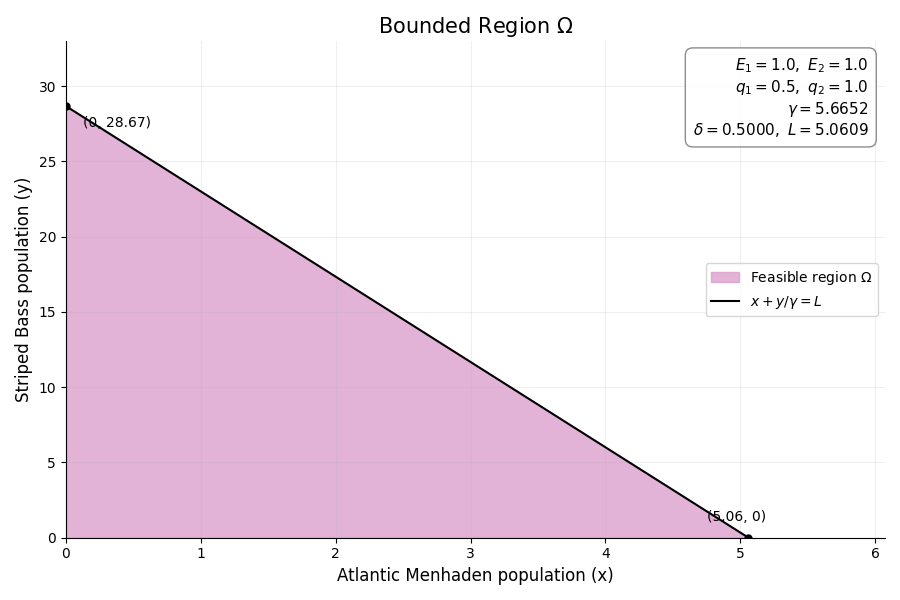
\includegraphics[width=0.85\textwidth]{images/region_omega.png}
    \caption{Minh họa miền giới hạn $\Omega$ của hệ với
    bộ tham số trong Bảng 1.}
    \label{fig:region_omega}
\end{figure}

\subsection{Xác định các điểm cân bằng của mô hình}
\label{subsec:bionomic_equilibrium}

Cân bằng sinh học--kinh tế đạt được khi quần thể của hai loài không còn thay đổi theo thời gian và tổng doanh thu từ hoạt động khai thác bằng tổng chi phí khai thác. Do đó, tại trạng thái cân bằng ta có
\[
\frac{dx}{dt}=0,
\qquad
\frac{dy}{dt}=0,
\qquad
\pi(E_1,E_2)=0.
\]

Giả sử điểm cân bằng sinh học--kinh tế có dạng
\[
P(x_B,y_B,E_{1B},E_{2B}),
\]
trong đó $x_B,y_B$ là kích thước quần thể của cá Atlantic Menhaden và Striped Bass; $E_{1B},E_{2B}$ là cường độ khai thác tương ứng tại trạng thái cân bằng.

\vspace{0.3cm}

Khi đó, điểm cân $P$ phải thỏa mãn hệ
\begin{equation}
\begin{cases}
r-ax-by-q_1E_1=0,\\[4pt]
-e-cy+dx-q_2E_2=0,\\[4pt]
(p_1q_1x-c_1)E_1+(p_2q_2y-c_2)E_2=0.
\end{cases}
\label{eq:bionomic_equilibrium_system}
\end{equation}

\subsubsection{Trường hợp 1: Chỉ khai thác cá Striped Bass (Vật săn mồi)}

Xét trường hợp $E_1=0$ và $E_2\neq 0$, tức hoàn toàn không khai thác cá Atlantic Menhaden (con mồi) .
Khi đó, phương trình lợi nhuận trong hệ
\eqref{eq:bionomic_equilibrium_system} trở thành
\[
(p_2q_2y-c_2)E_2=0.
\]

Vì $E_2\neq 0$, suy ra
\[
p_2q_2y-c_2=0
\quad\Longleftrightarrow\quad
y_B=\frac{c_2}{p_2q_2}.
\]

Thế $y_B$ vào phương trình thứ nhất của hệ \eqref{eq:bionomic_equilibrium_system}, ta được
\[
r-ax_B-by_B=0
\quad\Longleftrightarrow\quad
x_B=\frac{r}{a}-\frac{bc_2}{ap_2q_2}.
\]

Tiếp tục thế $x_B$ và $y_B$ vào phương trình thứ hai của hệ \eqref{eq:bionomic_equilibrium_system}, ta được:
\[
-e-cy_B+dx_B-q_2E_{2B}=0
\quad\Longleftrightarrow\quad
E_{2B}
=
-\frac{e}{q_2}
-
\frac{cc_2}{p_2q_2^2}
+
\frac{d}{q_2}
\left(
\frac{r}{a}
-
\frac{bc_2}{ap_2q_2}
\right).
\]

Do đó, điểm cân bằng sinh học--kinh tế trong trường hợp chỉ khai thác
Striped Bass là
\[
P_1
=
\left(
\frac{r}{a}-\frac{bc_2}{ap_2q_2},
\frac{c_2}{p_2q_2},
0,
E_{2B}
\right).
\]

Điểm cân bằng này tồn tại khi $x_B>0$ và $E_{2B}>0$, tương đương với:
\[
\frac{r}{a}>\frac{bc_2}{ap_2q_2},
\qquad
\frac{d}{q_2}
\left(
\frac{r}{a}-\frac{bc_2}{ap_2q_2}
\right)
>
\frac{e}{q_2}
+
\frac{cc_2}{p_2q_2^2}.
\]

\subsubsection{Trường hợp 2: Chỉ khai thác cá Atlantic Menhaden (con mồi)}

Xét trường hợp $E_1\neq 0$ và $E_2=0$, tức không khai thác cá Striped Bass (Vật săn mồi).
Khi đó, phương trình lợi nhuận trong hệ
\eqref{eq:bionomic_equilibrium_system} trở thành
\[
(p_1q_1x-c_1)E_1=0.
\]

Vì $E_1\neq 0$, suy ra
\[
p_1q_1x-c_1=0
\quad\Longleftrightarrow\quad
x_B=\frac{c_1}{p_1q_1}.
\]

Thế $x_B$ vào phương trình thứ hai của hệ
\eqref{eq:bionomic_equilibrium_system}, ta được
\[
-e-cy_B+dx_B=0
\quad\Longleftrightarrow\quad
y_B=
\frac{dc_1}{cp_1q_1}-\frac{e}{c}.
\]

Tiếp tục thế $x_B$ và $y_B$ vào phương trình thứ nhất của hệ
\eqref{eq:bionomic_equilibrium_system}, ta được
\[
r-ax_B-by_B-q_1E_{1B}=0
\quad\Longleftrightarrow\quad
E_{1B}
=
\frac{r}{q_1}
-
\frac{ac_1}{p_1q_1^2}
-
\frac{b}{q_1}
\left(
\frac{dc_1}{cp_1q_1}-\frac{e}{c}
\right).
\]

Do đó, điểm cân bằng sinh học--kinh tế trong trường hợp chỉ khai thác
Atlantic Menhaden là
\[
P_2
=
\left(
\frac{c_1}{p_1q_1},
\frac{dc_1}{cp_1q_1}-\frac{e}{c},
E_{1B},
0
\right).
\]

Điểm cân bằng này tồn tại khi $y_B>0$ và $E_{1B}>0$, tương đương với:
\[
\frac{dc_1}{cp_1q_1}>\frac{e}{c},
\qquad
\frac{r}{q_1}
-
\frac{ac_1}{p_1q_1^2}
>
\frac{b}{q_1}
\left(
\frac{dc_1}{cp_1q_1}-\frac{e}{c}
\right).
\]

\subsubsection{Trường hợp 3: Không khai thác cả hai loài}

Xét trường hợp $E_1=0$ và $E_2=0$, tức không khai thác cả Atlantic Menhaden (con mồi) và Striped Bass (vật săn mồi).

Khi đó, hệ \eqref{eq:bionomic_equilibrium_system} trở thành
\[
\begin{cases}
r-ax-by=0,\\
-e-cy+dx=0.
\end{cases}
\]

Đây là hệ phương trình bậc nhất hai ẩn $x$ và $y$. Giải hệ, ta thu được
\[
x^*
=
\frac{rc+be}{ac+bd},
\qquad
y^*
=
\frac{rd-ae}{ac+bd}.
\]

Do đó, điểm cân bằng sinh học trong trường hợp không khai thác cả hai loài là
\[
P_3
=
\left(
\frac{rc+be}{ac+bd},
\frac{rd-ae}{ac+bd},
0,
0
\right).
\]

Để điểm cân bằng có ý nghĩa sinh học, cần $x^*>0$ và $y^*>0$. 

Dễ dàng nhận thấy $x^*>0$ do các tham số đều dương. 

Mặt khác,
$y^*>0 \Longrightarrow rd>ae$.

Vì vậy, điểm cân bằng $P_3$ tồn tại nếu:
\[
rd>ae.
\]

\subsubsection{Trường hợp 4: Khai thác đồng thời cả hai loài}

Xét trường hợp $E_1\neq 0$ và $E_2\neq 0$, tức đồng thời khai thác cả Atlantic Menhaden (con mồi) và Striped Bass (vật săn mồi).

Giả sử chi phí khai thác không vượt quá doanh thu tương ứng
của mỗi loài, tức là
\[
    c_1 \leq p_1q_1x,\qquad c_2 \leq p_2q_2y.
\]
Khi đó, lợi nhuận từ mỗi hoạt động khai thác đều không âm:
\[
    p_1q_1x-c_1 \geq 0,\qquad p_2q_2y-c_2 \geq 0.
\]
Mặt khác, do $E_1>0$, $E_2>0$ và tổng lợi nhuận
tại trạng thái cân bằng sinh học--kinh tế bằng $0$, ta có
\[
    (p_1q_1x-c_1)E_1+(p_2q_2y-c_2)E_2=0.
\]
Vì tổng của hai số không âm bằng $0$ nên từng số
phải bằng $0$. Do đó,
\[
    \begin{cases}
        p_1q_1x-c_1=0,\\
        p_2q_2y-c_2=0
    \end{cases}
    \Longleftrightarrow
    \begin{cases}
        x_B=\dfrac{c_1}{p_1q_1},\\[6pt]
        y_B=\dfrac{c_2}{p_2q_2}.
    \end{cases}
\]

Khi đó, để phương trình lợi nhuận trong hệ
\eqref{eq:bionomic_equilibrium_system} bằng $0$, ta cần:
\[
p_1q_1x_B-c_1=0,
\qquad
p_2q_2y_B-c_2=0,
\]
suy ra
\[
x_B=\frac{c_1}{p_1q_1},
\qquad
y_B=\frac{c_2}{p_2q_2}.
\]

Thế $x_B$ và $y_B$ vào phương trình thứ nhất của hệ
\eqref{eq:bionomic_equilibrium_system}, ta được
\[
r-ax_B-by_B-q_1E_{1B}=0
\quad\Longleftrightarrow\quad
E_{1B}
=
\frac{r}{q_1}
-
\frac{ac_1}{p_1q_1^2}
-
\frac{bc_2}{p_2q_1q_2}.
\]

Tương tự, thế $x_B$ và $y_B$ vào phương trình thứ hai:
\[
-e-cy_B+dx_B-q_2E_{2B}=0
\quad\Longleftrightarrow\quad
E_{2B}
=
-\frac{e}{q_2}
-
\frac{cc_2}{p_2q_2^2}
+
\frac{dc_1}{p_1q_1q_2}.
\]

Do đó, điểm cân bằng sinh học--kinh tế trong trường hợp khai thác đồng thời cả hai loài là
\[
P_4
=
\left(
\frac{c_1}{p_1q_1},
\frac{c_2}{p_2q_2},
E_{1B},
E_{2B}
\right).
\]

Vì $x_B>0$ và $y_B>0$ khi các tham số đều dương, điểm cân bằng $P_4$ tồn tại khi
$E_{1B}>0$ và $E_{2B}>0$, tương đương với
\[
\frac{r}{q_1}
>
\frac{ac_1}{p_1q_1^2}
+
\frac{bc_2}{p_2q_1q_2},
\qquad
\frac{dc_1}{p_1q_1q_2}
>
\frac{e}{q_2}
+
\frac{cc_2}{p_2q_2^2}.
\]


\subsection{Phân tích tính ổn định và khả năng phục hồi của hệ sinh thái}

Để kiểm tra tính ổn định của hệ khi có hoạt động khai thác,
ta xét ma trận Jacobian:
\begin{equation}
    J(x,y)=
    \begin{pmatrix}
        r-2ax-by-q_1E_1 & -bx\\
        dy & -e-2cy+dx-q_2E_2
    \end{pmatrix}.
\end{equation}


Với ma trận Jacobian cấp hai, các trị riêng
là nghiệm của phương trình đặc trưng
\[
    \lambda^2-\operatorname{tr}(J)\lambda
    +\det(J)=0.
\]
Theo tiêu chuẩn Routh--Hurwitz, nếu
$\operatorname{tr}(J)<0$ và $\det(J)>0$
thì các trị riêng đều có phần thực âm,
suy ra điểm cân bằng ổn định tiệm cận.

Bên cạnh đó, để đánh giá khả năng
phục hồi sau nhiễu động nhỏ, xét thời gian hồi phục
đặc trưng $\tau$ và khả năng phục hồi $R$:
\begin{equation}
    \tau=-\frac{1}{\operatorname{Re}(\lambda_m)},
    \qquad R=\frac{1}{\tau},
\end{equation}
trong đó $\lambda_m$ là trị riêng có phần thực lớn nhất
của ma trận Jacobian tại điểm cân bằng ổn định.

\subsubsection{Trường hợp 1: Chỉ khai thác cá Striped Bass (Vật săn mồi)}

Xét trường hợp $E_1=0$, $E_2>0$. Tại điểm cân bằng
cùng tồn tại $(\hat{x},\hat{y})$, ta có
\[
    \begin{cases}
        a\hat{x}+b\hat{y}=r,\\
        d\hat{x}-c\hat{y}=e+q_2E_2.
    \end{cases}
\]

Giải hệ, ta thu được
\[
    \hat{x}=\frac{b(e+q_2E_2)+rc}{ac+bd},
    \qquad
    \hat{y}=\frac{rd-a(e+q_2E_2)}{ac+bd}.
\]

Vì $\hat{x}>0$, điều kiện $\hat{y}>0$ tương đương
\begin{equation}
    0\leq E_2<\frac{rd-ae}{aq_2}.
\end{equation}

Tại điểm cân bằng, ma trận Jacobian trở thành
\[
    J(\hat{x},\hat{y})=
    \begin{pmatrix}
        -a\hat{x} & -b\hat{x}\\
        d\hat{y} & -c\hat{y}
    \end{pmatrix}.
\]

Khi đó,
\[
    \operatorname{tr}(J)=-(a\hat{x}+c\hat{y})<0,
    \qquad
    \det(J)=(ac+bd)\hat{x}\hat{y}>0.
\]

Do đó, điểm cân bằng $(\hat{x},\hat{y})$ ổn định
tiệm cận với mọi $E_2$ thỏa mãn điều kiện trên.

Thời gian hồi phục $\tau(E_2)$ được xác định
từ trị riêng có phần thực lớn nhất của
$J(\hat{x}(E_2),\hat{y}(E_2))$.

Theo kết quả tính toán của mô hình, khi tăng $E_2$,
thời gian hồi phục ban đầu giảm, sau đó tăng mạnh
khi $E_2$ tiến gần ngưỡng khai thác tới hạn
\[
    E_{2,\mathrm{crit}}=\frac{rd-ae}{aq_2}.
\]
Tại ngưỡng này, $\hat{y}\to0^+$ và
$\tau(E_2)\to+\infty$.

% Chèn đồ thị tau(E2) tại đây sau khi vẽ bằng Python.
% \begin{figure}[htbp]
%     \centering
%     \includegraphics[width=0.85\textwidth]{tau_predator.png}
%     \caption{Thời gian hồi phục theo cường độ
%     khai thác Striped Bass.}
%     \label{fig:tau_predator}
% \end{figure}


\subsubsection{Trường hợp 2: Chỉ khai thác cá Atlantic Menhaden
(con mồi)}

Xét trường hợp $E_1>0$, $E_2=0$. Tại điểm cân bằng
cùng tồn tại $(\bar{x},\bar{y})$, ta có
\[
    \begin{cases}
        r-a\bar{x}-b\bar{y}=q_1E_1,\\
        -e-c\bar{y}+d\bar{x}=0.
    \end{cases}
\]

Giải hệ, ta thu được
\[
    \bar{x}=\frac{c(r-q_1E_1)+be}{ac+bd},
    \qquad
    \bar{y}=\frac{d(r-q_1E_1)-ae}{ac+bd}.
\]

Để điểm cân bằng cùng tồn tại có ý nghĩa sinh học,
cần $\bar{x}>0$ và $\bar{y}>0$.
Điều kiện $\bar{y}>0$ suy ra
\begin{equation}
    0\leq E_1<\frac{rd-ae}{dq_1}.
\end{equation}

Điều kiện này cũng bảo đảm $\bar{x}>0$.

Tại điểm cân bằng, ma trận Jacobian có dạng
\[
    J(\bar{x},\bar{y})=
    \begin{pmatrix}
        -a\bar{x} & -b\bar{x}\\
        d\bar{y} & -c\bar{y}
    \end{pmatrix}.
\]

Với
\[
    \operatorname{tr}(J)=-(a\bar{x}+c\bar{y})<0,
    \qquad
    \det(J)=(ac+bd)\bar{x}\bar{y}>0,
\]
suy ra điểm cân bằng $(\bar{x},\bar{y})$ ổn định
tiệm cận với mọi $E_1$ thỏa mãn điều kiện trên.

Thời gian hồi phục $\tau(E_1)$ tăng theo cường độ
khai thác và tiến tới vô hạn khi
\[
    E_1\to E_{1,\mathrm{crit}}^-,
    \qquad
    E_{1,\mathrm{crit}}=\frac{rd-ae}{dq_1}.
\]

% Chèn đồ thị tau(E1) tại đây.
% \begin{figure}[htbp]
%     \centering
%     \includegraphics[width=0.85\textwidth]{tau_prey.png}
%     \caption{Thời gian hồi phục theo cường độ
%     khai thác Atlantic Menhaden.}
%     \label{fig:tau_prey}
% \end{figure}


\subsubsection{Trường hợp 3: Khai thác đồng thời cả hai loài}

Xét trường hợp cả Atlantic Menhaden và Striped Bass
được khai thác với cùng cường độ $E_1=E_2=E$.
Tại điểm cân bằng cùng tồn tại $(x^*,y^*)$, ta có
\[
    \begin{cases}
        ax^*+by^*=r-q_1E,\\
        dx^*-cy^*=e+q_2E.
    \end{cases}
\]

Giải hệ, ta được
\[
    x^*=\frac{cr+be-(cq_1-bq_2)E}{ac+bd},
    \qquad
    y^*=\frac{rd-ae-(dq_1+aq_2)E}{ac+bd}.
\]

Để điểm cân bằng tồn tại và có ý nghĩa sinh học,
cần $x^*>0$, $y^*>0$.

Với $y^*$, ta có
\[
    y^*>0
    \Longleftrightarrow
    E<\frac{rd-ae}{dq_1+aq_2}.
\]

Đối với $x^*$, nếu $cq_1\leq bq_2$ thì
$x^*>0$ với mọi $E\geq0$. Ngược lại, nếu
$cq_1>bq_2$ thì
\[
    x^*>0
    \Longleftrightarrow
    E<\frac{cr+be}{cq_1-bq_2}.
\]

Do đó, điểm cân bằng cùng tồn tại có ý nghĩa sinh học khi
\[
    0\leq E<
    \begin{cases}
        \dfrac{rd-ae}{dq_1+aq_2},
        & cq_1\leq bq_2,\\[10pt]
        \min\left\{
            \dfrac{cr+be}{cq_1-bq_2},
            \dfrac{rd-ae}{dq_1+aq_2}
        \right\},
        & cq_1>bq_2.
    \end{cases}
\]

Thế $(x^*,y^*)$ vào ma trận Jacobian:
\[
    J(x^*,y^*)=
    \begin{pmatrix}
        -ax^* & -bx^*\\
        dy^* & -cy^*
    \end{pmatrix}.
\]

Khi đó,
\[
    \operatorname{tr}(J)=-(ax^*+cy^*)<0,
    \qquad
    \det(J)=(ac+bd)x^*y^*>0.
\]

Vì vậy, điểm cân bằng $(x^*,y^*)$ ổn định
tiệm cận với mọi $E$ thỏa mãn điều kiện tồn tại.

Với bộ tham số được sử dụng trong nghiên cứu,
$cq_1<bq_2$, nên ngưỡng khai thác được xác định bởi
\[
    E_{\mathrm{crit}}
    =\frac{rd-ae}{dq_1+aq_2}.
\]

Thời gian hồi phục $\tau(E)$ tăng theo cường độ
khai thác và tiến tới vô hạn khi
$E\to E_{\mathrm{crit}}^-$.

\subsubsection{Minh họa số}

Sử dụng bộ tham số sinh học đã được hiệu chỉnh
trong Bảng 1 cùng với $q_1=0.5$ và $q_2=1$,
ta minh họa quỹ đạo nghiệm và thời gian hồi phục
của hệ dưới các chế độ khai thác khác nhau.

Hình~\ref{fig:phase_portraits} biểu diễn chân dung pha
của hệ trong bốn trường hợp khai thác.
Các quỹ đạo nghiệm từ những điều kiện ban đầu khác nhau
có xu hướng hội tụ về điểm cân bằng cùng tồn tại,
minh họa tính ổn định tiệm cận của hệ.

\begin{figure}[htbp]
    \centering
    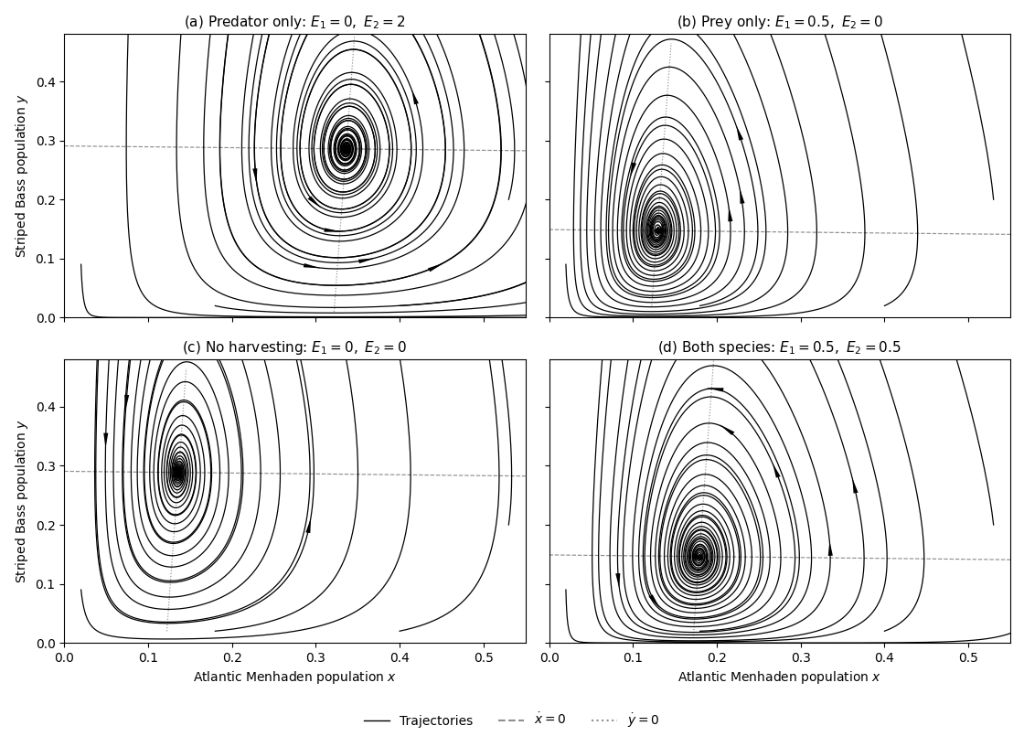
\includegraphics[width=\textwidth]{images/phase_potrait.png}
    \caption{Chân dung pha của hệ trong bốn trường hợp:
    (a) chỉ khai thác Striped Bass;
    (b) chỉ khai thác Atlantic Menhaden;
    (c) không khai thác;
    (d) khai thác đồng thời cả hai loài.}
    \label{fig:phase_portraits}
\end{figure}

Hình~\ref{fig:return_time} thể hiện sự phụ thuộc
của thời gian hồi phục $\tau$ vào cường độ khai thác.
Khi chỉ khai thác Striped Bass, thời gian hồi phục
ban đầu giảm rồi tăng mạnh gần ngưỡng tới hạn.
Ngược lại, khi khai thác Atlantic Menhaden hoặc
đồng thời cả hai loài, thời gian hồi phục tăng
theo cường độ khai thác.

\begin{figure}[htbp]
    \centering
    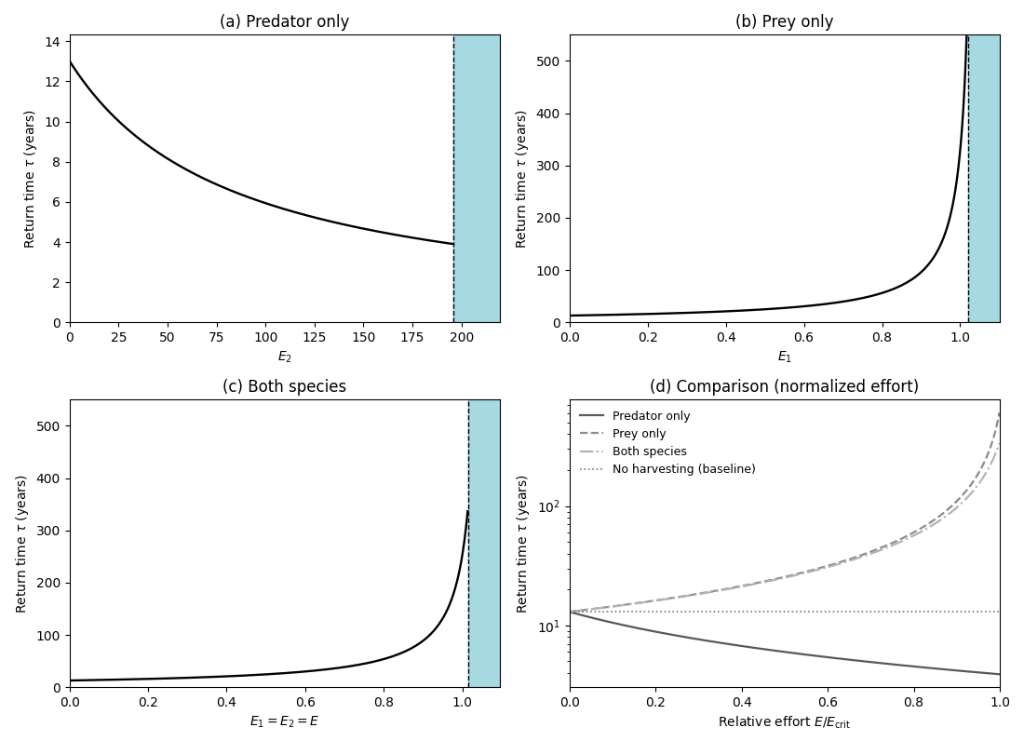
\includegraphics[width=\textwidth]{images/return_time.png}
    \caption{Sự phụ thuộc của thời gian hồi phục $\tau$
    vào cường độ khai thác:
    (a) chỉ khai thác Striped Bass;
    (b) chỉ khai thác Atlantic Menhaden;
    (c) khai thác đồng thời cả hai loài;
    (d) so sánh thời gian hồi phục theo cường độ
    khai thác được chuẩn hóa.}
    \label{fig:return_time}
\end{figure}



% Chương 4: Phân tích các chính sách khai thác nghề cá
\chapter{PHÂN TÍCH CÁC CHÍNH SÁCH KHAI THÁC NGHỀ CÁ}
\label{ch:policies}

\textit{(Nội dung chi tiết của chương này sẽ được phát triển đầy đủ trong giai đoạn tiếp theo):}

\section{Chính sách Sản lượng bền vững tối đa (MSY)}
\begin{itemize}
    \item Tối đa hóa hàm sản lượng đánh bắt $Y(E) = q_1 E x^* + q_2 E y^*$.
    \item \textbf{Trường hợp 1 (Chỉ khai thác cá vược sọc):} Nỗ lực $E_{\mathrm{MSY}} = \frac{rd - ae}{2aq_2}$. Chứng minh quần thể kẻ săn mồi ở mức MSY bằng 50\% quần thể khi chưa đánh bắt (Định lý 4.1).
    \item \textbf{Trường hợp 2 (Chỉ khai thác cá mòi dầu):} Điều kiện tồn tại MSY đòi hỏi $\frac{rd - ae}{cr + be} > \frac{d}{2c}$. Đối với hệ sinh thái vịnh Chesapeake, điều kiện này không thỏa mãn, nỗ lực $E_{Y_m} \approx 1.02$ sẽ dẫn tới sự tuyệt chủng của cá vược sọc; do đó chính sách khuyến nghị giảm 50\%: $E_{\mathrm{MSY}} = 0.5$ (Định lý 4.2).
    \item \textbf{Trường hợp 3 (Khai thác đồng thời cả hai loài):} Điều kiện tồn tại nghiệm bền vững và mức khuyến nghị an toàn sinh thái $E_{\mathrm{MSY}} = 0.5$ (Định lý 4.3).
\end{itemize}

\section{Chính sách Sản lượng kinh tế tối đa (MEY)}
\begin{itemize}
    \item Tối đa hóa hàm tô kinh tế ròng $\mathrm{Rent}(E) = R(E) - C(E) = \hat{p} Y(E) - \hat{c} E$.
    \item Chứng minh tính chất quan trọng: $E_{\mathrm{MEY}} < E_{\mathrm{MSY}}$ khi chỉ đánh bắt cá vược sọc, khẳng định chính sách MEY thân thiện hơn với bảo tồn sinh thái.
    \item Phân tích nghịch lý kinh tế khi đánh bắt cá mòi dầu hoặc cả hai loài trong vịnh Chesapeake: $E_{\mathrm{MEY}}$ nhận giá trị âm dưới các giả định chi phí thông thường, chứng minh MEY không thể áp dụng độc lập mà cần kết hợp bảo trợ hệ sinh thái.
\end{itemize}

\section{Chính sách Sản lượng tối đa hóa độ đàn hồi (RMY)}
\begin{itemize}
    \item Đánh giá tác động của nỗ lực khai thác lên độ hồi phục $R$ và thời gian cân bằng $\tau$.
    \item \textbf{Đánh bắt cá vược sọc:} Độ đàn hồi tăng tuyến tính theo nỗ lực trong miền khảo sát ($E_{\mathrm{RMY}} = 10$).
    \item \textbf{Đánh bắt cá mòi dầu:} Độ đàn hồi giảm đơn điệu ngặt theo $E_1$, đạt cực đại tại $E_1 = 0$; bất kỳ nỗ lực đánh bắt cá mòi dầu nào cũng phải trả giá bằng sự suy giảm độ bền vững sinh thái.
    \item \textbf{Đánh bắt kết hợp hai loài:} Sự đánh đổi gay gắt giữa sản lượng và độ ổn định hệ thống.
\end{itemize}


% Chương 5: Phân tích độ nhạy cục bộ
\chapter{PHÂN TÍCH ĐỘ NHẠY CỤC BỘ}
\label{ch:sensitivity}

\textit{(Nội dung chi tiết của chương này sẽ được phát triển đầy đủ trong giai đoạn tiếp theo):}

\section{Phương pháp vi phân trực tiếp (Direct Differential Method)}
\begin{itemize}
    \item Thiết lập hệ phương trình vi phân mở rộng gồm 2 phương trình trạng thái và các phương trình cho véctơ độ nhạy:
    \begin{equation}
    \frac{d}{dt}\left(\frac{\partial u_i}{\partial p_j}\right) = J \cdot S_j + F_j,
    \end{equation}
    với véctơ 8 tham số $p = (r, a, b, E_1, e, c, d, E_2)$.
    \item Tính ma trận Jacobian $J(x, y)$ và ma trận đạo hàm riêng của vế phải $F$.
\end{itemize}

\section{Chỉ số độ nhạy tương đối và xếp hạng tham số}
\begin{itemize}
    \item Tính chuẩn Euclidean của ma trận độ nhạy tương đối:
    \begin{equation}
    \|\bar{S}_{ij}\|_2 = \sqrt{\sum_{k=1}^N \left(\frac{\partial u_i}{\partial p_j}(t_k) \frac{p_j}{u_i(t_k)}\right)^2}.
    \end{equation}
    \item \textbf{Đối với cá vược sọc:} Nhạy cảm nhất với tốc độ tăng trưởng nội tại của cá mòi dầu $r$ ($\|\cdot\|_2 \approx 1.0080$), hệ số săn bắt $b$ ($\approx 1.0004$) và nỗ lực đánh bắt cá mòi dầu $E_1$ ($1.9647 E_1/q_1$).
    \item \textbf{Đối với cá mòi dầu:} Nhạy cảm nhất với hiệu suất chuyển hóa dinh dưỡng $d$ ($\approx 0.9985$), tỷ lệ tử vong tự nhiên của kẻ săn mồi $e$ ($\approx 0.8886$) và nỗ lực đánh bắt cá vược sọc $E_2$ ($0.7328 E_2/q_2$).
    \item Thảo luận ý nghĩa thực nghiệm đối với các nhà quản lý sinh thái.
\end{itemize}


% Chương 6: Thảo luận và Kết luận
\chapter{KẾT LUẬN VÀ KIẾN NGHỊ}
\label{ch:conclusion}

\textit{(Nội dung chi tiết của chương này sẽ được phát triển đầy đủ trong giai đoạn tiếp theo):}

\section{Tổng kết các kết quả đạt được}
\begin{itemize}
    \item Đã xây dựng và khảo sát toàn diện mô hình toán học Lotka--Volterra tổng quát 2 loài tích hợp yếu tố khai thác và kinh tế sinh thái cho hệ cá mòi dầu -- cá vược sọc tại vịnh Chesapeake.
    \item Đã chứng minh chặt chẽ tính đặt đúng của mô hình (tính dương và bị chặn toàn cục trong miền $\Omega$).
    \item Đã chỉ ra sự khác biệt bản chất và những hiểm họa tiềm ẩn khi áp dụng chính sách MSY đơn loài cho cá mồi; chứng minh sự cần thiết của việc giảm 50\% hạn ngạch đánh bắt cá mòi dầu để bảo vệ kẻ săn mồi.
    \item Đã phân tích tính khả thi và giới hạn của chính sách MEY và RMY đối với hệ thống đa loài.
    \item Đã định lượng mức độ nhạy cảm của các tham số then chốt thông qua phương pháp vi phân trực tiếp.
\end{itemize}

\section{Hàm ý chính sách quản lý cho vịnh Chesapeake}
\begin{itemize}
    \item Chuyển đổi căn bản từ quản lý đơn loài sang Quản lý Nghề cá Dựa trên Hệ sinh thái (EBFM).
    \item Thiết lập các Điểm tham chiếu sinh thái (ERP) nghiêm ngặt đối với cá mòi dầu Đại Tây Dương để bảo tồn nguồn thức ăn cho cá vược sọc và các loài thủy sản thượng tầng.
    \item Kiểm soát chặt chẽ đội tàu lưới vây công nghiệp và hạn ngạch của các tập đoàn đánh bắt lớn.
\end{itemize}

\section{Đánh giá hạn chế và hướng phát triển tiếp theo}
\begin{itemize}
    \item Mô hình hiện tại chưa xét đến cấu trúc tuổi (\textit{age-structured models}) và kích thước cá thể.
    \item Cần mở rộng mô hình sang mạng lưới nhiều hơn 2 loài (kết hợp cá xanh, cá yếu, sinh vật phù du và các loài chim di cư).
    \item Tích hợp các yếu tố môi trường ngẫu nhiên (\textit{stochastic differential equations}) và tác động của biến đổi khí hậu trong các nghiên cứu mở rộng tiếp theo.
\end{itemize}


% --- TÀI LIỆU THAM KHẢO ---
\newpage
\addcontentsline{toc}{chapter}{TÀI LIỆU THAM KHẢO}
\bibliographystyle{plain}
\bibliography{references}

\end{document}
